\cotefile{137}
\scanpage{45}
% archive foliation: 44
produits $\prod$ aussi --- ce qui est \unsure{automatique} si le $K^\bullet$ est nul sauf en nb fini\unsure{...}]

\deleted{Comme le \unsure{foncteur} $\operatorname{Hom}_{\unsure{k}}^\bullet(K_{\unsure{i}}^\bullet,C^\bullet)$
$(\unsure{B}^\circ\longrightarrow(Ab))$ \unsure{définit} un \unsure{fonct.} additif des
$K$, \unsure{il est représentable par} $K^\bullet$.}

\unsure{Définissons} un hom dans $\widehat{\unsure{B}}$
\[
(1)\qquad F(x)\unsure{\longrightarrow|=}\operatorname{Hom}_{\unsure{k}}^\bullet(\unsure{K^\bullet|K}(x),C_F^\bullet)
=\operatorname{Hom}_{\unsure{k}}^\bullet(\unsure{K|K^\bullet}(x),F(C^\bullet))
\]
i.e. un hom dans $\widehat{\unsure{B}}^\bullet$
\[
(1')\qquad \underbrace{F(x)\otimes\unsure{k}^\bullet(x)}_{\unsure{resp.}}\longrightarrow C^\bullet=F(C^\bullet)
\]
\margin{\unsure{repr. en les} $\unsure{x}$\unsure{,} \unsure{d'où}\unsure{\simeq} \unsure{l'isom. de V.f.}}
\[
(1'')\qquad
\underset{\substack{\rotatebox{90}{$\in$}\\\widehat{\unsure{B}}}}{F(x)}
\otimes\underset{\substack{\rotatebox{90}{$\in$}\\Ab_{\unsure{k}}^\bullet}}{\operatorname{Hom}(x,C^\bullet)}
\xrightarrow[\mathrm{can}]{}F(C^\bullet)
\]
qui provient de l'hom fonctoriel en $x\in\operatorname{Ob}\unsure{K}$
\[
F(x)\otimes\operatorname{Hom}(x,C)\longrightarrow F(C).
\]
L'hom (1''), donc (1) est fonctoriel en $K$,
et les deux membres sont des foncteurs
additifs en $K$, pour prouver que \unsure{(1)}
est un iso, $\forall F$, il suffit de le voir
pour $K$ de la forme $\unsure{les} C^{\unsure{i|\bullet}}$. Or on a
alors
\[
(2)\qquad F(C^{\unsure{i|\bullet}})\longrightarrow\operatorname{Hom}_{K}^\bullet
(C_{\unsure{\bullet}}^{\unsure{i|\bullet}},\deleted{\unsure{C}}F(C^\bullet))
\]
Or on a aussi un
\[
\operatorname{Hom}_{\unsure{k}}^\bullet
\left(C_{\unsure{\bullet}}^{\unsure{i|\bullet}},\underset{\substack{\rotatebox{90}{$\in$}\\Ab^\bullet}}{P^\bullet}\right)
\simeq C^{\unsure{i|\bullet}}
\]
et on voit de suite que moyennant cet is.,
(2) va à l'identité, qfd.

\scanpage{46}
% archive foliation: 45
\margin{\uline{NB} Le foncteur $DP^*$ \unsure{défini de façon} \unsure{fidèle} dans $B$ additive (\unsure{par les sommes}).}
\uline{Ex 3} La théorie de Dold-Puppe nous donne
une \deleted{\unsure{équivalence de catégories}} \inserted{équivalence de catégories}
(pour les catégories \deleted{$\unsure{Ab}_k^\bullet$} $Ab_k$ additives avec facteurs directs)
\margin{$ND={}$\unsure{non dégénéré}\\ $DP={}$\unsure{Dold-Puppe} \deleted{\unsure{catégorie de} $Ab$}}
\diagram{\begin{tikzcd}
B_\bullet \arrow[r,phantom,"\simeq" description] \arrow[r,shift right=.7ex,"DP^*"'] & B_* \arrow[l,shift right=.7ex,"ND_\bullet"']
\end{tikzcd}}
donc aussi (en \unsure{appliquant à} $B^\circ$)
\diagram{\begin{tikzcd}
B^\bullet \arrow[r,phantom,"\simeq" description] \arrow[r,shift right=.7ex,"DP_*"'] & B^* \arrow[l,shift right=.7ex,"ND^\bullet"']
\end{tikzcd}}
\margin{\unsure{Isom.} compatibles aux fonct. additifs.}
en particulier
\[
Ab_{\unsure{k}\bullet}\simeq Ab_{k*},\qquad Ab_k^\bullet\simeq Ab_k^*.
\]
\deleted{Il est immédiat \illegible{1}.}
L'image essentielle de $K_\bullet^{\unsure{k}}$ et $K_{\unsure{k}}^\bullet$ par ces
deux foncteurs sont notés $K_*$ et $K^*$.
\margin{$k$ est \unsure{sous-entendu dans les notations}, \unsure{sinon} c'est $K_\bullet(k)$ \unsure{avec indices ou exposants} $\bullet$ ou $*$.}
On a donc un diagramme d'équivalences
canoniques
\diagram{\begin{tikzcd}[row sep=large,column sep=large]
\deleted{\unsure{Ab_{k\bullet}}}\arrow[r,shift right=.6ex,"\deleted{DP}"'] &
\deleted{\unsure{Ab_{k*}}}\arrow[l,shift right=.6ex,"\deleted{ND}"']\\
\deleted{Ab_k^\bullet}\arrow[r,shift right=.6ex] &\deleted{Ab_k^*}\arrow[l,shift right=.6ex]
\end{tikzcd}}
\margin{Convention d'écriture. Pour un objet $C$ de $K$,
on note $C_\bullet,C_*,C^\bullet,C^*$ les objets correspondants
obtenus en appliquant $\alpha_\bullet,\alpha_*,\alpha^\bullet,\alpha^*$, et les
comp. sont notés $C_n,C_{[n]},C^n,C^{[n]}$
(\unsure{Attention}, ne pas oublier les signes $[\ ]$
et $C_\bullet,C_*,C^\bullet,C^*,C$).}
\diagram{\begin{tikzcd}[row sep=large,column sep=large]
K_\bullet \arrow[rr,shift right=.7ex,"DP^*"']
\arrow[dd,leftrightarrow,"\underset{\circ}{\vee}\ \deleted{\unsure{\mathrm{inv}}}"'] &&
K_* \arrow[ll,shift right=.7ex,"ND_\bullet"']
\arrow[dd,leftrightarrow,"\underset{\circ}{\vee}\ \deleted{\unsure{\mathrm{inv}}}"]\\
&K\arrow[ul,"\alpha_\bullet"]\arrow[ur,"\alpha_*"]
\arrow[dl,"\underset{\circ}{\alpha^\bullet}"']\arrow[dr,"\underset{\circ}{\alpha^*}"]&\\
K^\bullet\arrow[rr,shift right=.7ex,"DP_*"']&&K^*\arrow[ll,shift right=.7ex,"ND^\bullet"']
\end{tikzcd}}
Les flèches \deleted{\unsure{ainsi}} marquées d'un signe
$\circ$ sont des foncteurs \uline{contravariants}.

On a

\uline{Proposition 4} \deleted{\unsure{de (C)}} On a tjs un
hom canonique

\scanpage{47}
% archive foliation: 46
\[
\alpha_*(C_\bullet^i)\simeq DP(C_\bullet^i)\simeq\bigwedge^{i+1}\Phi_*
\]
\[
(\text{d'où}\qquad \alpha^*(C_i^\bullet)\simeq DP(C_i^\bullet)\simeq\bigwedge^{i+1}\unsure{\Phi_*|\Phi^*}\quad)
\]
\deleted{\unsure{L'obj. déf.} de $\alpha(C_\bullet^i)$ est \unsure{l'image} de $\unsure{T}_{*\wedge}$
par le foncteur $ND:K_*\longrightarrow K_\bullet$ \unsure{donné} \unsure{can.}
de $(\bigwedge^{\geqslant1})\unsure{\Phi}_*$.}
\deleted{\unsure{Par suite}}
\deleted{\uline{Cor. 1} Le foncteur $DP:Ab_{k\bullet}\longrightarrow\unsure{Ab}$}

Appliquant la théorie de Dold-Puppe à $K$
\deleted{(qui est bien additive et stable par facteurs
directs, au moins si $k$ est principal, p.ex.
$k=\mathbf Z$)} on trouve dans $K$ un complexe
\[
\deleted{\unsure{C}}\qquad C^*=DP(C^\bullet)
\]
(\unsure{qu'on} \deleted{\unsure{pourra prendre}} \unsure{a donc défini} dans \deleted{$\unsure{K}$} $K(k)$ \unsure{quelque}
\unsure{part soit} $k$), d'où pour les $B$ $k$-additives
\diagram{\begin{tikzcd}[row sep=large,column sep=large]
\underline{\operatorname{Hom}}_{k\text{-lin}}(K,B)\arrow[d,"\simeq"',"\mathrm{rest}"]
\arrow[ddr,bend left=18,"F\longmapsto F(C^*)"]&\\
\underline{\operatorname{Hom}}_{k\text{-lin}}(\unsure{A},B)\arrow[d,"\simeq"',"F\longmapsto F(C^\bullet)"]&\\
B^\bullet\arrow[r,"DP",hook]&B^*
\end{tikzcd}}
donc un foncteur $F\longmapsto F(C^*)$ qui est pl. fid.
Si $B$ est karoubienne, $DP_B$ est une équivalence,
donc aussi $F\longmapsto F(C^*)$. Donc
$C^*$ apparait comme objet simplicial \uline{universel}
dans cat. $k$-additive karoubienne.

\uline{Prop 5} Si $B$ est $k$-additive karoubienne, alors
$F\longmapsto F(C^*)$ est une équivalence
\[
\underline{\operatorname{Hom}}_{k\text{-lin}}(K,B)\longrightarrow B^*.
\]
(On a un \unsure{hom|sens} canoniquement \inserted{\unsure{bif. de}}
$F\in\operatorname{Ob}\underline{\operatorname{Hom}}_{k\text{-lin}}(K,B)$ et $x\in\operatorname{Ob}K$.
\margin{\unsure{i}}

\scanpage{48}
% archive foliation: 47
\margin{\unsure{?|2}}

\scanpage{49}
% archive foliation: 48
\margin{Il vaut mieux construire $\unsure{\mathcal P|P}$ ``en l'air'', puis les \unsure{noter}
$\unsure{\mathcal P|P}_\bullet,\unsure{\mathcal P|P}_*,\unsure{\mathcal P|P}^\bullet,\unsure{\mathcal P|P}^*$ comme pour $K$.}
Soit $\unsure{\mathcal P|P}_\bullet$ la catégorie des complexes de $k$-chaines $L_\bullet$
qui sont libres de \unsure{t.f.|r.f.} en chaque dim,
et qui n'ont qu'un nb fini de composantes
non nulles. Une suite :
\[
0\unsure{-|\longrightarrow}L'_\bullet\unsure{-|\longrightarrow}L_\bullet\unsure{-|\longrightarrow}L''_\bullet\longrightarrow0
\]
\inserted{d'hom dans $\unsure{\mathcal P|P}_\bullet$} est dite exacte spéciale, si $\forall n\geqslant0$, la suite
\[
0\longrightarrow L'_n\longrightarrow L_n\unsure{-|\longrightarrow}L''_n\longrightarrow0
\]
est \unsure{ex. ab.} Soit $\Sigma_\bullet$ la
classe de ces suites. Ainsi $\unsure{\mathcal P|P}_\bullet$ est muni de
$C_\bullet^\bullet$ (complexe de cochaines) et de $\Sigma_\bullet$. On va
voir que, pour ces données, il est sol. d'un
pb universel.
\margin{!}

Soit \deleted{$\unsure{B}$} $B$ une cat. additive. Un ens. $\Sigma$ de
suites
\[
(*)\qquad 0\unsure{-|\longrightarrow}A'\xrightarrow{q}A\xrightarrow{p}A''\unsure{-|\longrightarrow}0
\]
dans $B$ est dit ``une classe de suites exactes''
si elle satisfait aux conditions

Sex 1) Si $(*)\in\Sigma$, alors $A'\xrightarrow{\sim}\operatorname{Ker}p$, $\operatorname{Coker}q\xrightarrow{\sim}A''$,
i.e. les suites $0\unsure{-|\longrightarrow}A'\unsure{-|\longrightarrow}A\longrightarrow A''$ et \deleted{\unsure{les}}
$A'\unsure{-|\longrightarrow}A\longrightarrow A''\unsure{-|\longrightarrow}0$
sont exactes (i.e. $\forall B\in\operatorname{Ob}B$, les suites de groupes
ab.
\[
\left\{\begin{aligned}
0&\unsure{-|\longrightarrow}\operatorname{Hom}(B,A')\unsure{-|\longrightarrow}\operatorname{Hom}(B,A)\unsure{-|\longrightarrow}\operatorname{Hom}(B,A'')\\
0&\unsure{-|\longrightarrow}\operatorname{Hom}(A'',B)\unsure{-|\longrightarrow}\operatorname{Hom}(A,B)\unsure{-|\longrightarrow}\operatorname{Hom}(A',B)
\end{aligned}\right.
\]
\deleted{\unsure{et}} sont exactes.

Sex 2) $\Sigma$ stable par iso, par sommes finies
et contient les suites de la forme
\[
0\unsure{-|\longrightarrow}A\xrightarrow{\mathrm{id}}A\unsure{-|\longrightarrow}0\unsure{-|\longrightarrow}0
\]
\[
0\unsure{-|\longrightarrow}0\unsure{-|\longrightarrow}A\xrightarrow{\mathrm{id}}A\longrightarrow0
\]
(donc aussi les suites de la forme
\[
0\unsure{-|\longrightarrow}A\xrightarrow{\mathrm{inj}}A\times B\xrightarrow{\mathrm{pr.}}B\unsure{-|\longrightarrow}0\qquad)
\]

\scanpage{50}
% archive foliation: 49
Un $\Sigma$-monomorphisme (épimorphisme)
$A\longrightarrow B$ de $B$ est un morphisme qui s'insère
dans une suite $\in\Sigma$
\[
0\unsure{-|\longrightarrow}A\unsure{-|\longrightarrow}B\longrightarrow K\longrightarrow0
\quad(\text{resp. }0\unsure{-|\longrightarrow}\unsure{\mathcal P|P}\unsure{-|\longrightarrow}A\longrightarrow B\longrightarrow0).
\]
Un morphisme \inserted{$A\longrightarrow B$} est $\Sigma$-strict s'il a un
noyau $\unsure{\mathcal P|P}$ et un conoyau $Q$, \inserted{\unsure{et si} $\operatorname{Coim}u\unsure{\xrightarrow{\sim}|\longrightarrow}\operatorname{Im}u$}
(et si $\unsure{\mathcal P|P}\longrightarrow A$, $(B\longrightarrow Q)$ est un $\Sigma$-mono ($\Sigma$-épi)), il
revient au même de dire que l'on peut trouver
des suites $\in\Sigma$
\margin{\unsure{déf. de} $\Sigma$-\unsure{strict}.}
\[
\begin{aligned}
0&\unsure{-|\longrightarrow}\unsure{\mathcal P|P}\longrightarrow A\longrightarrow R\longrightarrow0\\
0&\unsure{-|\longrightarrow}R\longrightarrow B\longrightarrow Q\longrightarrow0
\end{aligned}
\]
telles que $A\longrightarrow B$ soit le composé $A\longrightarrow R\longrightarrow B$.
(Il faut peut-être exiger qu'un composé de
$\Sigma$-mono (resp. $\Sigma$-épi) est idem.)

On définit de façon évidente les \inserted{objets} $\Sigma$-projectifs
et $\Sigma$-injectifs. Une \deleted{suite \unsure{complexe de cocha. (chaines)}}
\deleted{$\cdots\longrightarrow C^{i-1}\longrightarrow C^i\longrightarrow C^{i+1}\longrightarrow\cdots$}
\deleted{est dit spécial.}
\[
A\xrightarrow{u}B\xrightarrow{v}C
\]
est dite \deleted{\unsure{spéciale si}} \inserted{$\Sigma$-spéciale} \deleted{\unsure{dès}} si elle
\deleted{\unsure{s'insère dans un diagramme} \unsure{exact}}
\inserted{$vu=0$, $u$ et $v$ stricts et \unsure{si l'on a}}
la suite exacte $\in\Sigma$
\diagram{\begin{tikzcd}[column sep=small,row sep=small]
0\arrow[r]&\operatorname{Ker}u\arrow[r]&A\arrow[r]&\operatorname{Coim}u\arrow[r]\arrow[d,equal]&0&&&&\\
&&0\arrow[r]&\operatorname{Im}u\arrow[r]&\operatorname{Ker}v\arrow[r]\arrow[d,equal]&H\arrow[r]&0&&\\
&&&0\arrow[r]&\operatorname{Ker}v\arrow[r]&B\arrow[r]&\operatorname{Coim}v\arrow[r]\arrow[d,equal]&0&\\
&&&&&0\arrow[r]&\operatorname{Im}v\arrow[r]&C\arrow[r]&\unsure{\operatorname{Coker}v}\arrow[d]\\
&&&&&&&&\unsure{0}
\end{tikzcd}}
(c'est une notion autoduale) On dit qu'un
complexe $C^\bullet$ dans $B$ est \uline{$\Sigma$-spécial} si \unsure{...},
\uline{$\Sigma$ acyclique} si \uline{de plus} les $H^i(C^\bullet)$ sont nuls,
une $\Sigma$-résolution si c'est un complexe
de cochaines ($C^i=0$ si $i<0$) et
$H^i=0$ pour $i\unsure{>|\neq}0$.

\scanpage{51}
% archive foliation: 50
Il faudrait prouver le
\margin{!}
\uline{Th.} Soit $B$ une cat. \deleted{add.} $k$-additive munie d'une
famille $\Sigma$ de suites exactes,
\margin{\unsure{nb. faut-il supposer} \unsure{que} $B$ cat. abélienne
($\Sigma$ \unsure{des suites ex.})}
$\underline{\operatorname{Hom}}_{k,\Sigma\text{-ex}}(\unsure{\mathcal P|P}_\bullet,B)$ la \inserted{$k$-}catégorie \deleted{pleine de}
$\underline{\operatorname{Hom}}_k(\unsure{\mathcal P|P}_\bullet,B)$ formée des foncteurs $\Sigma$-exacts,
i.e. transformant suites de $\Sigma_\bullet$ en suites de $\Sigma$,
\deleted{\unsure{désignons les foncteurs exacts}}
\deleted{$\unsure{\underline{\operatorname{Hom}}}_{\Sigma\text{-ex}}(\unsure{\mathcal P|P}_\bullet,B)$ la sous-catégorie pleine}
$\underline{\operatorname{Hom}}_{k,\Sigma\text{-lex}}(\unsure{\mathcal P|P}_\bullet,B)$ la sous-catégorie pleine de
celles qui \deleted{transforment \unsure{les noyaux en noyaux}}
\inserted{commutent aux $\Sigma$-noyaux}.

a) Le foncteur restriction $F\longmapsto F(C_\bullet^\bullet)$
\[
\underline{\operatorname{Hom}}_{k,\Sigma\text{-\unsure{lex|ex}}}(\unsure{\mathcal P|P}_\bullet,B)
\longrightarrow\deleted{\underline{\operatorname{Hom}}_{k\text{-lin}}(K,B)=}B^\bullet
\]
\deleted{est une équivalence de catégories}
\inserted{est pleinement fidèle,}
\deleted{(\unsure{pour le foncteur} \unsure{sur} $\underline{\operatorname{Hom}}_{k,\Sigma\text{-lex}}$)}
l'image essentielle est
formée des $C^\bullet\in\operatorname{Ob}B^\bullet$ tels que les
$d^i:C^i\longrightarrow C^{i+1}$ admettent des \inserted{$\Sigma$-}\unsure{noyaux}.
\margin{\unsure{est une équivalence de cat.}}
[donc \deleted{$\unsure{K}$} $(\unsure{\mathcal P|P}_\bullet,C_\bullet^\bullet,\Sigma_\bullet)$ est universel pour
les triples $(B,C^\bullet,\Sigma)$ tels que
les $d^i:C^i\longrightarrow C^{i+1}$ aient des $\Sigma$-noyaux, quand
on prend comme morphismes les
foncteurs \deleted{\unsure{commutant}} $\Sigma$-exacts à g.]

b) Le foncteur \deleted{induit} \inserted{$F\longmapsto F(C_\bullet^\bullet)$}
\[
\underline{\operatorname{Hom}}_{k,\Sigma\text{-ex}}(\unsure{\mathcal P|P}_\bullet,B)\longrightarrow B^\bullet
\]
(qui est pl. fid. par a)) a comme
image essentielle les $C^\bullet\in\operatorname{Ob}B^\bullet$ qui sont
des $\Sigma$-résolutions (i.e. $\Sigma$-spéciaux et
avec $H^i(C^\bullet)=0$ si $i>0$).
\deleted{[donc le triple $(\unsure{\mathcal P|P}_\bullet,C_\bullet^\bullet,\Sigma_\bullet)$ apparait comme
universel pour les $(B,C^\bullet,\Sigma)$ tels que
$C^\bullet$ soit \unsure{une} $\Sigma$-résolution, --- les}

\scanpage{52}
% archive foliation: 51
\deleted{foncteurs admissibles étant maintenant
les foncteurs $\Sigma$-exacts.)}
\deleted{\uline{Indications sur dém.}
Dans $\unsure{\mathcal P|P}_\bullet$, il est évident que \uline{$C_\bullet^\bullet$ est une}
\uline{$\Sigma_\bullet$-spéciale résolution}. De façon précise,
si
\[
\unsure{\longrightarrow|-}\Psi_\bullet^i=\deleted{\unsure{H}(C_\bullet^i)\longrightarrow}\ k\deleted{[i]}\text{ placé en degré }i
\]
on voit que $\unsure{\Psi_\bullet^{-1}}=0$, et des suites $\in\Sigma_\bullet$
\[
\begin{aligned}
0&\unsure{-|\longrightarrow}\Psi_\bullet^0\longrightarrow C_\bullet^0\longrightarrow\Psi_\bullet^1\unsure{-|\longrightarrow}0\\
&\qquad0\longrightarrow\Psi_\bullet^1\unsure{-|\longrightarrow}C_\bullet^1\longrightarrow\Psi_\bullet^2\longrightarrow0\\
&\qquad\qquad0\unsure{-|\longrightarrow}\Psi_\bullet^2\unsure{-|\longrightarrow}C_\bullet^2\unsure{-|\longrightarrow}\Psi_\bullet^3\longrightarrow0.
\end{aligned}
\]
De plus, on voit que pour $L_\bullet\in\operatorname{Ob}\unsure{\mathcal P|P}_\bullet$,
$L_\bullet$ peut s'écrire comme extension successive
d'objets de la forme $(\Psi_\bullet^i)^{\unsure{r_i|\rho_i}}$ pour la
filtration croissante
\[
\operatorname{Fil}_i(L_\bullet)_j=\begin{cases}L_j&\text{si }j\leqslant i\\0&\text{si }j>i\end{cases}
\]
on a un isom can
\[
\deleted{\unsure{Fil}}\operatorname{Gr}_i(L_\bullet)\simeq L_i\text{ placé en degré }i
\underset{\mathrm{can}}{\simeq}\Psi_\bullet^i\otimes L_i
\underset{\text{non can}}{\simeq}(\Psi_\bullet^i)^{\unsure{r_i|\rho_i}}
\]
\uline{Enfin}, les \deleted{$\unsure{Q}$} $C_\bullet^i$ sont $\Sigma_\bullet$-projectifs.
Soit $B^\bullet_{\Sigma\text{-\unsure{nex|lex}}}$ (resp. $B^\bullet_{\Sigma\text{-ex}}$) les sous-catégories
pleines de $B^\bullet$ décrites dans a) (resp. b)).
On va définir des foncteurs
}
\diagram{\begin{tikzcd}[row sep=large,column sep=large]
\deleted{B^\bullet_{\Sigma\text{-\unsure{nex|lex}}}}\arrow[r]\arrow[d,hook]&
\deleted{\underline{\operatorname{Hom}}_{\Sigma\text{-\unsure{lex}}}(\unsure{\mathcal P|P}_\bullet,B)}\arrow[d,hook]\\
\deleted{B^\bullet_{\Sigma\text{-ex}}}\arrow[r]&
\deleted{\underline{\operatorname{Hom}}_{\Sigma\text{-ex}}(\unsure{\mathcal P|P}_\bullet,B)}
\end{tikzcd}}
\deleted{(le premier induisant le deuxième)}

\scanpage{53}
% archive foliation: 52
\deleted{Soit $\unsure{\mathcal P|P}\supset K$ une sous-catégorie $k$-additive.}
\diagram{\begin{tikzcd}
\deleted{\underline{\operatorname{Hom}}_{k\text{-lin}}(\unsure{\mathcal P|P},B)}\arrow[r,shift left=.6ex,"\deleted{\rho}"]&
\deleted{B}\arrow[l,shift left=.6ex,"\deleted{\sigma}"]
\end{tikzcd}}
\margin{\deleted{$B$ cat. additive avec $\Sigma$ classe de suites exactes et $\Sigma$-noyaux.}}
\margin{\deleted{\unsure{\phi}}}
\diagram{\begin{tikzcd}
\deleted{\underline{\operatorname{Hom}}_{k\text{-lin}}(\unsure{\mathcal P|P},\widehat B)}\arrow[d,"\deleted{\vee}"]&\\
\deleted{\underline{\operatorname{Hom}}_{k\text{-lin}}(\unsure{\mathcal P|P},B)}\arrow[r,"\deleted{\rho}"]&
\deleted{B^\bullet}\arrow[ul,"\deleted{\sigma}"']
\end{tikzcd}}

$B$ catégorie additive, \deleted{avec noyaux et \unsure{fibres|filtres}}
\deleted{\unsure{une} $\Sigma$ de suites exactes}, où
$\forall$ morphisme admet un $\Sigma$-noyau
\diagram{\begin{tikzcd}[column sep=large]
\underline{\operatorname{Hom}}_{k,\Sigma\text{-\unsure{lex}}}(\unsure{\mathcal P|P}_\bullet,B)
\arrow[r,shift left=.6ex,"\rho"]&B^\bullet\arrow[l,shift left=.6ex,"\sigma"]
\end{tikzcd}}
\margin{non, il faut condition de platitude ?}
cat. des foncteurs $k$-lin
$F:\unsure{\mathcal P|P}\longrightarrow B$
qui transforment suites $\in\Sigma$
en suites exactes à g.
\[
\left\{\begin{aligned}
\rho(F)&=F(C^\bullet)\\
\sigma(C^\bullet)(L_\bullet)&\simeq\underbrace{\operatorname{Hom}_{k}^\bullet(L_\bullet^\vee,C^\bullet)}_{
\substack{\text{défini grâce à l'existence}\\\text{des }\Sigma\text{-noyaux}}}
\simeq\operatorname{Hom}_k^\bullet(\operatorname{Hom}(L_\bullet,C_\bullet^\bullet),C^\bullet)
\end{aligned}\right.
\]
Formule d'adjonction
\diagram{\begin{tikzcd}[row sep=small,column sep=large]
\operatorname{Hom}(\rho(F),C^\bullet)\arrow[r,"\simeq"]\arrow[d,equal]&\operatorname{Hom}(F,\sigma(C^\bullet))\\
\operatorname{Hom}(F(C^\bullet),C^\bullet)&
\end{tikzcd}}
Le deuxième ens est formé des hom fonctoriels en $L_\bullet$
\[
F(L_\bullet)\longrightarrow\operatorname{Hom}_k^\bullet(L_\bullet^\vee,C^\bullet)
\]
\inserted{$L^\bullet$}
i.e. des hom ``fonctoriels en $L_\bullet$''
\[
L^\bullet\otimes_k F(L_\bullet)\longrightarrow C^\bullet.
\]
Or on a $L^\bullet\simeq\operatorname{Hom}(L_\bullet,C_\bullet^\bullet)$
\[
F(L)\otimes L^\bullet\deleted{\otimes F(L_\bullet)}\simeq
\operatorname{Hom}(L_\bullet,C_\bullet^\bullet)\otimes F(L_\bullet)\xrightarrow{\mathrm{taut.}}F(C^\bullet)
\]
et on trouve qu'on a ainsi la ``\deleted{\unsure{fonctorialité}}''
compatibilité à l'op. diff. en $L^\bullet$ et $C^\bullet$, et ``\unsure{fonctorialité}''

\scanpage{54}
% archive foliation: 53
en $L_\bullet$'', ce qui donne si on veut
\[
F\xrightarrow{u}\sigma\rho F
\]
hom fonctoriel en $F$, \uline{\unsure{d'où}} \deleted{\unsure{la}} \unsure{l'hom|l'un}
d'adjonction postulée
\diagram{\begin{tikzcd}[row sep=large,column sep=large]
\operatorname{Hom}(\rho F,C^\bullet)\arrow[rr]\arrow[dr,dashed]&&\operatorname{Hom}(F,\sigma C^\bullet)\\
&\operatorname{Hom}(\sigma\rho F,\sigma C^\bullet)\arrow[ur,"\alpha\longmapsto\alpha\circ u"']&
\end{tikzcd}}
à prouver que c'est un iso --- vérification
facile.

L'hom can
\[
\rho\sigma C^\bullet\unsure{-|\longrightarrow}C^\bullet
\]
est un iso, i.e. $\sigma$ est pl. fid. En effet,
\[
\rho(\sigma(C^\bullet))=\sigma(C^\bullet)(C_\bullet^\bullet)
=\left(\underbrace{\sigma(C^\bullet)(C_\bullet^i)}_{\substack{
\operatorname{Hom}_k^\bullet(C_i^\bullet,C^\bullet)\\\Vert\\C^i}}
\right)_i\simeq(C^i)_i\quad\mathrm{OK}.
\]
Ainsi on a une inclusion pl. fidèle
\[
B^\bullet\mathrel{\mathop{\hookrightarrow}\limits^{\sigma}}\underline{\operatorname{Hom}}_{k,\Sigma\text{-\unsure{sex|lex}}}
\subset\underline{\operatorname{Hom}}_{k\text{-lin}}
\]
où $\Sigma$-\unsure{sex|lex} désigne les foncteurs qui transforment
suites de $\Sigma$ en suites exactes à g.

Quelle est l'image essentielle de $B^\bullet$ ?
(On donnera des exemples \unsure{tantôt de|quantité de}
foncteurs dans l'image ess.) est-ce tout
$\underline{\operatorname{Hom}}_{k,\Sigma\text{-\unsure{sex|lex}}}$ ? Elle est formée des $F$
tels que
\[
F\xrightarrow{u}\sigma\rho(F)
\]
soit un iso. Or on a

\scanpage{55}
% archive foliation: 54
\[
F(C_\bullet^i)\unsure{-|\longrightarrow}\sigma(\rho(F))(C_\bullet^i)
=\operatorname{Hom}_k^\bullet(C_i^\bullet,\underbrace{\rho(F)}_{\Vert\;F(C_\bullet^\bullet)})
\simeq F(C_\bullet^i)
\]
\[
\begin{aligned}
F(\Psi_\bullet^i)&\longrightarrow\operatorname{Hom}_k^\bullet(\Psi_i^\bullet,F(C_\bullet^\bullet))
\simeq Z^i(F(C_\bullet^\bullet))\\
&\simeq\operatorname{Ker}(F(C_\bullet^i)\longrightarrow F(C_\bullet^{i+1}))\\
&\simeq F(\underbrace{\operatorname{Ker}(C_\bullet^i\unsure{-|\longrightarrow}C_\bullet^{i+1})}_{\Sigma\text{-Ker !}})
=F(\Psi_\bullet^i).
\end{aligned}
\]
Donc on voit que $u(L_\bullet):F(L_\bullet)\longrightarrow\sigma\rho(F)(L_\bullet)$
est un iso sur les $C_\bullet^i$ et les $\Psi_\bullet^i$ donc
sur \deleted{\unsure{toute}} la cat. additive $\unsure{\mathcal P|P}_0\supset K$ des sommes
de tels.) Pour avoir $\forall L_\bullet$, on \unsure{raisonne}
\inserted{\unsure{ess. par}}
par récurrence sur la longueur $n$ \deleted{\unsure{de $L_\bullet$}},
\inserted{de l'intervalle $[p,q]$ tel que $L_i=0$ si $i\notin[p,q]$.}
C'est vrai si $n=0$, ($L_\bullet$ somme $\simeq(\Psi_\bullet^i)^r$
\deleted{\unsure{$i>0$}}), on
suppose $n>0$ et suppose que c'est fait pour
$n-1$.
\diagram{\begin{tikzcd}[column sep=small,row sep=large]
&&\cdots\arrow[r]&0\arrow[r]&L_p\arrow[r,"\mathrm{id}"]&L_p\arrow[r]&0
&\left.\vphantom{\begin{matrix}L_p\\L_p\end{matrix}}\right\}
& (C_\bullet^{\unsure{p|p+1}})^r\;\deleted{\unsure{L_\bullet''}}\\
\cdots\arrow[r,dash]&0\arrow[r,dash]&L_{p+n}\arrow[r]&L_{p+n-1}\arrow[r,dashed]&L_{p+1}\arrow[u,"d_{p+1}"]\arrow[r]&L_p\arrow[u,"\mathrm{id}"]\arrow[r]&0\arrow[r]&0&L_\bullet\arrow[u]\\
&&&\underbrace{\hspace{5.8em}}_{\text{tronqué }L_\bullet'}&&&&&
\end{tikzcd}}
on trouve un \unsure{morph.} de suites exactes (où $L_p\simeq k^r$)
\diagram{\begin{tikzcd}[column sep=small,row sep=large]
0\arrow[r,dash]&(\Psi_\bullet^p)^r\arrow[r,dash]\arrow[d,equal]&L_\bullet\arrow[r]\arrow[d]&\deleted{\unsure{\Psi}}L_\bullet'\arrow[r]\arrow[d]&0\\
0\arrow[r]&(\Psi_\bullet^p)^r\arrow[r,dash]&(C_\bullet^p)^r\arrow[r,dash]&(\Psi_\bullet^{p+1})^r\arrow[r,dash]&0
\end{tikzcd}}
qui exprime $L_\bullet$ comme produit fibré
de $L_\bullet'$ et $(C_\bullet^p)^r$ sur $(\Psi_\bullet^{p+1})^r$ (i.e. comme
noyau d'un hom \inserted{$\Sigma$-\uline{épi}}
\[
(C_\bullet^p)^r\times L_\bullet^{\unsure{1|'}}\unsure{-|\longrightarrow}(\Psi_\bullet^{p+1})^r).
\]
Donc on conclut par

\scanpage{56}
% archive foliation: 55
l'hyp de récurrence. Cela donne donc
\[
\underline{\operatorname{Hom}}_{k,\Sigma\text{-sex}}(\unsure{\mathcal P|P}_\bullet,B)\xrightarrow{\sim}B^\bullet
\]
(si $B$ muni d'une \deleted{catégorie}\inserted{classe $\Sigma_0$} de suites exactes
telle que $\forall$ morphisme de $B$ admette
un $\Sigma$-noyau).

\uline{NB} Si on \inserted{ne} suppose \deleted{\unsure{plus} que $B$ admette une
classe $\Sigma$ de suites exactes, mais} \unsure{pas autre que}
$\forall$ morphisme de $B^\bullet$ admette un noyau,
l'argument donné montre seulement que
le foncteur ci-dessus $F\longmapsto F(C_\bullet^\bullet)$
\diagram{\begin{tikzcd}
\underline{\operatorname{Hom}}_{k,\Sigma\text{-sex}}(\unsure{\mathcal P|P}_\bullet,B)\arrow[r,shift right,"\rho"']&B^\bullet\arrow[l,shift right,"\sigma"']
\end{tikzcd}}
est pl. fid. (avec adjoint $\sigma$ comme dessus,
mais à valeurs dans $\underline{\operatorname{Hom}}_{k,\mathrm{lin}}(\unsure{\mathcal P|P}_\bullet,\widehat B)$);
on a néanmoins $\sigma\rho\simeq\mathrm{id}$ i.e.
\[
\deleted{F(L_\bullet)\simeq}\qquad
F(L_\bullet)\simeq\operatorname{Hom}_k^\bullet(L^\bullet,\underbrace{F(C_\bullet^\bullet)}_{\Vert\;C^\bullet})
\]
pour $\forall F\in\underline{\operatorname{Hom}}_{k,\Sigma\text{-sex}}$.

\uline{Re NB} On \deleted{\unsure{en}} vérifie facilement, sous les
conditions du NB, que si $F\longmapsto C^\bullet=F(C_\bullet^\bullet)$
se correspondent ($F\in\operatorname{Ob}\underline{\operatorname{Hom}}_{k,\Sigma\text{-sex}}$), alors
$F$ est $\Sigma$-\unsure{ex.act|ex.} ssi $C^\bullet$ est une $\Sigma_0$-résolution.
(du moins si $B$ cat. abélienne avec $\Sigma$ ttes
les suites exactes\ldots)

\uline{Ex} Soit $\unsure{\lambda|\Lambda}_\bullet\in\mathrm{Ab}_{k\bullet}$, considérons
\inserted{$\unsure{\mathcal P|P}_\bullet\unsure{-|\longrightarrow}\mathrm{Ab}_k$}
le foncteur $L_\bullet\longmapsto\operatorname{Hom}_{\mathrm{Ab}_{k\bullet}}(\lambda_\bullet,L_\bullet)$.
Il est $\Sigma$-exact à g (et même exact \uline{à g}) --- en fait
\margin{\unsure{TSVP}}

\scanpage{57}
% archive foliation: 56
la vérification de la formule
\[
\operatorname{Hom}_{\unsure{\bullet}}(\lambda_\bullet,L_\bullet)
\xrightarrow{\sim}\operatorname{Hom}(L_\bullet^\vee,\lambda_\bullet^\vee)
\]
est élémentaire.

\scanpage{58}
% archive foliation: 57
Construction \unsure{intrinsèque} de $\unsure{\mathcal P|P}$ ($k$-lin.)
$\unsure{\mathcal P|P}\supset K$, \unsure{et|en} satisfaisant les conditions

a) Le foncteur covariant
\[
L\longmapsto\operatorname{Hom}(L,C^0)^\vee
\]
est représentable par un \inserted{objet} $\Psi^0$.
\unsure{Consid.} l'hom $\Psi^0\unsure{-|\longrightarrow}C^0$ transposé de
\diagram{\begin{tikzcd}[column sep=large]
\operatorname{Hom}(\Psi^0,L)&\operatorname{Hom}(C^0,L)\arrow[l]&\bigl[\,\operatorname{Hom}(C^1,L)\arrow[l]\\
\operatorname{Hom}(L,C^0)^\vee\arrow[u,phantom,"\simeq" description,sloped]&&
\end{tikzcd}}
déduit de l'accouplement
\[
\begin{aligned}
\operatorname{Hom}(C^0,L)\times\operatorname{Hom}(L,C^0)&\unsure{-|\longrightarrow}\operatorname{Hom}(C^0,C^0)\simeq k\\
(u,\qquad v)&\longmapsto vu
\end{aligned}
\]
\diagram{\begin{tikzcd}[column sep=small,row sep=small]
&C^0\arrow[dl,"d"']\arrow[dr,"u"]&\\
C^1\arrow[rr,"u'"']&&L\arrow[dr,"v"]\\
&&&C^0
\end{tikzcd}}
Or si $u':C^1\unsure{-|\longrightarrow}L$, considérons
$u=u'\circ d^0$, et $v\circ u=v\circ(u'\circ d)$,
\inserted{$=(v\circ u')\circ d$}
comme on $v\circ u'=0$, on a donc $vu=0$, donc
le composé est
\[
\operatorname{Hom}(\Psi^0,L)\longleftarrow\operatorname{Hom}(C^0,L)
\unsure{-|\longleftarrow}\operatorname{Hom}(C^1,L)
\]
\margin{\unsure{Rem.|$\unsure{\mathcal P|P}$}}
\unsure{bien nul} ce qui signifie aussi que
\[
\Psi^0\longrightarrow C^0\unsure{-|\longrightarrow}C^1
\]
est nul, donc que $C^\bullet$ est $\Psi^0$-augmenté.
Soit $\unsure{\Phi^\bullet}$ le complexe de cochaînes qu'il forme.
\margin{\unsure{foncteur}
\diagram{\begin{tikzcd}[column sep=small,row sep=small]
\unsure{\unsure{\mathcal P|P}}\arrow[r]&\unsure{\operatorname{Hom}(\Phi^\bullet,\,)}\\
\unsure{L}\arrow[ur,maps to]&
\end{tikzcd}}}
\deleted{Notons aussi que}

\deleted{b) La famille des $C^i$ et $\Psi^0$ est génératrice \unsure{stricte}.}
\deleted{c) $\unsure{\Phi^\bullet}$ est une résolution de}
\inserted{(soit $\unsure{\mathcal P|P}_0$ la ss cat. \unsure{additive},
$k$-lin. \deleted{\unsure{eng.}} formée de sommes finies
d'objets de la forme $C^i$, $\Psi^0$, i.e. les
expressions de la forme
\[
L\oplus(\Psi^0)^r\qquad r\in\mathbf N,\ L\in\operatorname{Ob}K.
\]}

\margin{\unsure{pour b)}\quad\unsure{On a}}
b) Les suites
\[
0\unsure{-|\longrightarrow}L'\longrightarrow L\deleted{\unsure{\longrightarrow L''\longrightarrow0}},
\inserted{(0\longrightarrow L'\longrightarrow L\longrightarrow L''),}
\]
\inserted{$0\longrightarrow L\longrightarrow L''\longrightarrow0,\quad L'\unsure{-|\longrightarrow}L\unsure{-|\longrightarrow}L''\longrightarrow0$}
telles que les $\unsure{I|i}\in\unsure{\mathcal P|P}_0$ \unsure{soient proj. et|soit proj. et}
\unsure{pour celles} \unsure{i.e. telles que} $0\unsure{-|\longrightarrow}L'\unsure{-|\longrightarrow}L\unsure{-|\longrightarrow}L''\longrightarrow0$ soit exactes
\deleted{\unsure{pour les deux}}, sont exactes.
\margin{\figure{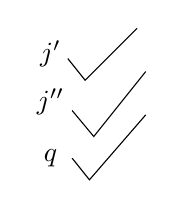
\begin{tikzpicture}[x=0.55cm,y=0.55cm]
\node at (0,2.4) {$\unsure{j'}$};\node at (0,1.3) {$\unsure{j''}$};\node at (0,0) {$\unsure{q}$};
\draw (0.4,2.3)--(0.8,1.8)--(2,3);\draw (0.5,1.1)--(1,0.5)--(2.2,2);\draw (0.5,0)--(0.9,-0.5)--(2.2,1);
\end{tikzpicture}}}
Soit $\Sigma$ la classe de ces suites

\deleted{\unsure{d)}} c) Le complexe augmenté $(C^\bullet,\Psi^0,\varepsilon)$ est
une $\Sigma$-résolution, i.e. $\unsure{\Phi^\bullet}$ est $\Sigma$-acyclique.

\scanpage{59}
% archive foliation: 58
% Manuscript written upside down relative to the supplied scan.
\deleted{Il faut prouver que \deleted{le noyau} l'hom}
\[
\deleted{\operatorname{Hom}_k^\bullet(L^\bullet,C^\bullet)\longrightarrow
Z^n(C^\bullet)^{\unsure{p|\beta}}\subset(C^n)^{\unsure{p|\beta}}}
\]
\deleted{admet un $\Sigma$-noyau}
\diagram{\begin{tikzcd}[column sep=large,row sep=large]
&\deleted{\underline{\operatorname{Hom}}_{\Sigma\text{-sex}}}\arrow[d]&\\
&\deleted{B^\bullet}\arrow[dl,bend right=15]\arrow[dr,bend right=12]&\\
\deleted{\underline{\operatorname{Hom}}_{\Sigma\text{-ex}}\simeq B^{\mathrm{rés}}}\arrow[ddr,bend right=15]&&\deleted{\underline{\operatorname{Hom}}_{\mathrm{sex}}\deleted{\unsure{\mathrm{pl}}}}\arrow[d,bend right=12]\\
&&\deleted{B^{\bullet\mathrm{pl}}\deleted{\unsure{\underline{\operatorname{Hom}}_{\mathrm{sex}}}}}\\
&\deleted{B^{\mathrm{rés.pl}}}&
\end{tikzcd}}
\margin{\deleted{$\left\{\begin{array}{l}B\text{ cat. abélienne}\\\Sigma\text{ suites exactes}\\\text{ordinaires}\end{array}\right.$}}
\[
\deleted{\operatorname{Ext}^1(L^\bullet,M)\Longleftarrow0}
\]
\[
\deleted{\underline{\operatorname{Hom}}_{\Sigma\text{-ex}}(\unsure{\mathcal P|P},B)
\overset{\sim}{\unsure{-|\longrightarrow}}\underline{\operatorname{Hom}}_{\Sigma\text{-ex}}(\unsure{\mathcal P|P}_0,B)}
\]
\deleted{$\unsure{\forall|N} B$ \deleted{\unsure{cat. de}}\inserted{admet}
(\inserted{$\Sigma$-}noyaux)}

\scanpage{60}
% archive foliation: 59
\unsure{Cela} signifie que l'on a une kyrielle de
suites $\Sigma$-exactes (donc exactes)
\diagram{\begin{tikzcd}[column sep=small,row sep=large]
0\arrow[r,dash]&\Psi^0\arrow[r]&C^0\arrow[r,dash]&\Psi^1\arrow[r,dash]&0&&&\\
&&0\arrow[r,dash]&\Psi^1\arrow[r,dash]&C^1\arrow[r]&\Psi^2\arrow[r]&0&\\
&&&&0\arrow[r]&\Psi^2\arrow[r,dash]&C^2\arrow[r,dash]&\Psi^3\arrow[r,dash]&0\\
&&&&&&\cdots&&
\end{tikzcd}}
Par hyp on sait que
\[
\Psi_\bullet^i=k\text{ placé en dim }i
\]
On trouve aisément les \deleted{\unsure{$\operatorname{Hom}(\Phi$}}\inserted{hom} entre les
$C^i$, et \deleted{\unsure{$\operatorname{Hom}($ les}} $\Psi^j$
\margin{\unsure{résulte de}\quad\unsure{par a)}}
\[
C^i\unsure{-|\longrightarrow}\Psi^j,\quad\Psi^i\unsure{-|\longrightarrow}C^j,\quad
\Psi^i\longrightarrow\Psi^j\qquad(C^i\unsure{-|\longrightarrow}C^j\text{ déjà connus})
\]
on peut résumer la situation en
disant que sur la sous-cat. str. pleine
$\unsure{\mathcal P|P}_1\subset\unsure{\mathcal P|P}$ formée des objets isom. à des sommes
des $C^i$ et des $\Psi^{\unsure{i|j}}$, le foncteur $L\longmapsto L_\bullet=
\operatorname{Hom}(\Phi^{\unsure{i|\bullet}},L)$ est pl. fidèle. Son image essentielle
est formée des complexes de chaînes $L_\bullet$
finis tels que les composantes \inserted{$L_i$, les $Z_i$ et les $B_i$}
\deleted{\unsure{$H_i(L)$}} soient libres de \unsure{t.f.|d.f.}

(On peut voir que le \deleted{\unsure{triplet|biplet}} $(\unsure{\mathcal P|P}_1,C^\bullet,\Psi^0,\varepsilon,\unsure{\Sigma\cap\unsure{\mathcal P|P}_1})$
est universel pour une cat. $k$-additive
munie d'une \uline{classe} $\Sigma$ de suites exactes et
d'une $\Sigma$-résolution d'un objet \deleted{$\Psi^0$} $Z^0$\ldots).

On va maintenant supposer de plus

d) Pour tte suite \inserted{$\Sigma$-}exacte de $\unsure{\mathcal P|P}$
\[
0\unsure{-|\longrightarrow}\unsure{L^\beta|L}\unsure{-|\longrightarrow}M\unsure{-|\longrightarrow}N\unsure{-|\longrightarrow}0
\]
\margin{il suffit de demander \unsure{l'une des deux propriétés}, par ex. \unsure{d)}}
et tout hom $L\unsure{-|\longrightarrow}L'$ (resp $N'\unsure{-|\longrightarrow}N$),
la suite \deleted{\unsure{nouvelle}} déduite par somme amalga-
mée (resp. produit fibré) existe dans $\unsure{\mathcal P|P}$

\scanpage{61}
% archive foliation: 60
et est $\Sigma$-exacte

(Variante : si $L\xrightarrow{u}M$ \deleted{est un $\Sigma$-épi},
\deleted{\unsure{dont le noyau}}
$\operatorname{Hom}(\Phi^i,u)$ sont épi $\forall i$ (i.e. $u_i:L_i\unsure{-|\longrightarrow}M_i$
épi) alors $u$ \deleted{\unsure{d'ailleurs}} admet un noyau
(donc on a une suite $\Sigma$-exacte
\[
0\unsure{-|\longrightarrow}\unsure{\mathcal P|P}\unsure{-|\longrightarrow}L\unsure{-|\longrightarrow}M\longrightarrow0\qquad).
\]
Utilisant ceci, on construit des objets
de $\unsure{\mathcal P|P}$ par ext. successives d'objets
$(\Psi_{\unsure{k}}^i)^{\unsure{r_i}}$ --- et on voit que $L\longmapsto L_\bullet=
\operatorname{Hom}(\Phi^\bullet,L)$ est \unsure{ess.} surjectif.

e) Tout objet de $\unsure{\mathcal P|P}$ est extension successive
d'objets de la forme $\Psi^i$ [qu'on peut
supposer \unsure{se succéder} par \unsure{ordre} croissant, dans
une filtration croissante \deleted{\unsure{de $\unsure{\mathcal P|P}$}}\inserted{\unsure{d'un objet} $L$},
laquelle sera alors canonique.]

\unsure{Je dois|Il doit} y avoir assez maintenant
pour conclure que le foncteur
$L\longmapsto L_\bullet=\operatorname{Hom}(\Phi^\bullet,L)$ est pl. fid. et
a l'image essentielle les $L_\bullet$ tels
que les $L_i,Z_i,B_i,H_i$ soient libres \unsure{t.f.}
et \inserted{$L_i$} nuls sauf un nb fini.

\scanpage{62}
% archive foliation: 61
\uline{Remarque} Supposons le \unsure{pt préc.} Alors
la catégorie $\unsure{\mathcal P|P}\simeq\unsure{\mathcal P|P}_\bullet$ \deleted{\unsure{est ab.}} admet des $\Sigma$-
noyaux (et des \unsure{Conoyaux}, mais un
bimorphisme n'est pas néc. un iso). \deleted{Je}
\deleted{\unsure{On fera attention que les mono}}
c'est \unsure{tjs|donc} vrai que si $N$ est le noyau
de $A\unsure{-|\longrightarrow}B$, alors $N\unsure{-|\longrightarrow}A$ est un $\Sigma$-
mono, i.e. s'insère dans une suite $\Sigma$-exacte
$0\longrightarrow N\unsure{-|\longrightarrow}A\unsure{-|\longrightarrow}A'\unsure{-|\longrightarrow}0$; mais le mono
$A'\unsure{-|\longrightarrow}B$ ne sera pas en général un
$\Sigma$-mono. Aussi on ne peut interpréter
$(\unsure{\mathcal P|P},\deleted{\unsure{\Psi^0}},C^\bullet,\deleted{\unsure{\Phi^\bullet,\varepsilon}}\inserted{\Sigma})$
comme \unsure{sol. d'un} \unsure{Pb} universel en appliquant tels quels les
développements précédents.

\deleted{Mais, \deleted{\unsure{d'autre part}}\inserted{on peut} généraliser
de façon naturelle, pour une
$B$ $k$-linéaire, la notion d'objet plat,}
\deleted{\unsure{et alors}} le syst. ci-dessus est universel
pour les $B$ \inserted{$k$-additives}, \unsure{munis} d'un complexe
de cochaînes \deleted{$\unsure{C^\bullet}$, et d'une \deleted{\unsure{ss}}\inserted{classe} $\Sigma$
de suites exactes, telle que tt hom
\inserted{$u:A\unsure{-|\longrightarrow}B$} de $B$ ait un noyau tel que
$\operatorname{Ker}u\longrightarrow A$ soit $\in\Sigma$}
$C^\bullet$ et d'une classe
$\Sigma_C$ de suites exactes, telle que tt
morphisme $u:A\unsure{-|\longrightarrow}B$ de $B$ admette
un noyau $K$ tel que $K\unsure{-|\longrightarrow}A$ soit un
$\Sigma_C$-mono : (on \unsure{prend} comme
\unsure{morphismes entre tels syst. ceux qui}
\unsure{transforme|transforment} $C^\bullet$ en $C'^\bullet$ et qui
\unsure{soit|sont} $\Sigma$-exact \uuline{à g}).

\scanpage{63}
% archive foliation: 62
On travaille dorénavant dans la catégorie $\unsure{\mathcal P|P}_1=Q$ (équivalente à la catégorie $Q_\bullet$ des complexes de chaînes finis où les $L_i,Z_i,B_i,H_i$ sont libres de type fini), \inserted{munie de $\Sigma_1=\Sigma\cap \unsure{\mathcal P|P}_1$}, dont la sous-catégorie des $\Sigma$-projectifs est \deleted{\unsure{add}} la catégorie \inserted{additive} $\unsure{\mathcal P|P}_0$ engendrée par les $C^i$ et $\Psi^0$ (i.e. par les $\Phi^i$), et celle des $\Sigma$-injectifs est la sous-cat. additive $K$ \deleted{\unsure{des sommes}} \inserted{engendrée} par les $C^i$ (les $L_\bullet$ \deleted{flasques} acycliques, i.e. les $L_*$ flasques\unsure{\ldots}). On s'intéresse aux \uline{résolutions droites} \inserted{$K^\bullet$} \uline{$\Sigma$-injectives de $\Psi^0$}, (i.e. des résolutions flasques $K_*^\bullet$ de $\unsure{k_\Delta|k_*}$ \inserted{$\unsure{\Psi}$} \unsure{---} (ce qui donnera \inserted{\unsure{donc}} en top Algébrique, des méthodes de calcul remarquables de la coh à coeff dans $k$). On a l'algèbre homologique ``relative'' aux classes des suites exactes, qui nous disent que si (comme c'est le cas ici) tout objet \deleted{\unsure{ad}} se plonge dans un $\Sigma$-injectif, \deleted{de façon} par un $\Sigma$-mono, alors \deleted{les \unsure{telles|deux} résolutions sont canoniques \unsure{à un}} deux résolutions sont homotopes, et il y a une seule classe d'homotopie d'hom de l'une dans l'autre (\uline{NB} Il y a aussi assez de projectifs, et on a l'énoncé analogue pour les résolutions projectives; on fera attention que les cat. $K$ des sommes de $C^i$ en

\scanpage{64}
% archive foliation: 63
contient pas \uline{assez} de \inserted{$\Sigma$-}projectifs: il faut y rajouter $\Psi^0$\ldots) \deleted{Il est vrai que} Ces assertions sont d'ailleurs vraies aussi dans la plus gde catégorie $\unsure{\mathcal P|P}$ [détermination des \inserted{$\Sigma$-}proj et des $\Sigma$-inj, et le fait qu'il y en a assez].

Les $\operatorname{Ext}^i$ calculés par les résolutions injectives \inserted{à droite} ou projectives \inserted{à g.} \deleted{\unsure{sont} (à gauche} \unsure{ou les} deux simultanément, sont les \unsure{mêmes} pour $i\geq1$, ce sont les hyperext habituels de \inserted{$L_\bullet$ et de $M_\bullet$}, (pour $i=0$ on doit prendre les $\unsure{L^i|L^\bullet}$.

Si $F:\ Q=\unsure{\mathcal P|P}_1\subset \unsure{\mathcal P|P}\ \unsure{\longrightarrow|{-}}\ B$ (\unsure{$k$-addit.}) \deleted{est un} foncteur, on peut construire les foncteurs dérivés \inserted{à droite et à g.} (en utilisant des résolutions injectives ou projectives.

Nous sommes intéressés notamment aux $R^iF(\Psi^0)$, qu'on note aussi $\unsure{\mathcal H^i(F)|H^i(F)}$ [on doit pouvoir montrer que ce sont les dérivés \inserted{droits} de $F\mapsto F(\Psi^0)=\Gamma(F)$, quand $F$ varie dans la cat. des \deleted{foncteurs} \inserted{$k$-add.} $\unsure{\mathcal P|P}\unsure{\longrightarrow|{-}}B$ \inserted{$\Sigma$-}exacts à gauche; (Si on se restreint à de tels $F$); \unsure{qu’elle|en effet} cette catégorie est équivalente à \deleted{\unsure{celle}} \deleted{$\unsure{B}$} $\unsure{B^\bullet|B'}$, $F\mapsto F(\Psi^0)$ s'identifie \deleted{alors} au foncteur $C^\bullet\mapsto Z^0(C^\bullet)$\inserted{$=H^0(C^\bullet)$} sur $\unsure{B^\bullet|B'}$, dont les dérivés sauf erreur sont les $H^i(C^\bullet)$ pour $i\geq1$. On a aussi $RF(\Psi^0)\simeq F(C^\bullet)$

\scanpage{65}
% archive foliation: 64
(\unsure{Ds.} la cat. dérivée) puisque $C^\bullet$ est une résolution $\Sigma$-injective de $\Psi^0$.

\figure{\begin{tikzpicture}[x=1cm,y=1cm]\draw (0,0) .. controls (-.5,-.6) and (-1.3,-.2) .. (-.9,.1) .. controls (-.5,.25) and (.8,.12) .. (1.4,.24);\end{tikzpicture}}

Nous considérons maintenant les réalisations $\tfrac12$ simpliciales $\unsure{\mathcal P|P}_*\supset Q_*\supset \unsure{\mathcal P|P}_{0*}\supset K_*\ \unsure{\text{etc.}}$ de $\unsure{\mathcal P|P}\supset Q\supset \unsure{\mathcal P|P}_0\supset K$. Sur $\unsure{\mathcal P|P}_*$ il y a la structure $\unsure{\otimes_k|\otimes_*}$ ou $\otimes_*$
($L_*\otimes_*M_*$ défini composante par composante
\[
(L_*\otimes M_*)_{[n]}=L_{[n]}\otimes M_{[n]}
\]
)
avec contraintes d'ass, unité ($\Psi^0$), et de comm, \inserted{\unsure{de bilinéar.}} \deleted{Il est quasi évident} \inserted{On note que $K_*$ est un} \deleted{(\unsure{bidirectionnel}) $\unsure{\mathcal P|P}^*,Q^*$,} ``co-idéal'', \deleted{que $\unsure{\mathcal P|P}_0$ est un \unsure{idéal}} \inserted{(i.e. si l'un des facteurs} $L_*,M_*$ est dans $K_*$, \unsure{l'autre aussi}), $\unsure{\mathcal P|P}_0$ et $Q$ sont stables par $\otimes$, car

\margin{\deleted{$\unsure{K}$} \unsure{Il s'agit} de $\unsure{\Psi_*}$ \unsure{qui sont} \unsure{contractiles} (\unsure{dualité})}

\diagram{\begin{tikzcd}[column sep=small,row sep=small]
\Psi^0_* \arrow[d,equal] & \otimes & \Psi^0_* \arrow[d,equal] & \simeq & \Psi^0_* \arrow[d,equal] & (\Rightarrow\text{ stabilité de }\unsure{\unsure{\mathcal P|P}_0})\\
\mathbf1_* && \mathbf1_* && \mathbf1_*
\end{tikzcd}}

et
\[
\Psi^i_*\otimes\Psi^j_*\simeq\Psi^{i+j}_*+\text{élém de }K
\]
\[
(\Rightarrow\text{ stabilité de }\unsure{\unsure{\mathcal P|P}_{1*}=Q})
\]

On transporte cette structure multiplicative sur $\unsure{\mathcal P|P}$ et ses sous-catégories (notation $*$, pour éviter des confusions) et sur autres réalisations $\unsure{\mathcal P|P}_\bullet$ et $\unsure{\mathcal P|P}^*,\unsure{\mathcal P|P}^\bullet$ (ces deux dernières contravariantes). On note $*$ sur $\unsure{\mathcal P|P}_\bullet$ et $\unsure{\mathcal P|P}^\bullet$, et $\unsure{\otimes|\mathbin{\circledast}}$ sur $\unsure{\mathcal P|P}^*$, car l'équivalence $\vee$ de

\scanpage{66}
% archive foliation: 65
$\unsure{\mathcal P|P}_*$ avec $\unsure{\mathcal P|P}^*$ est compatible aux $\otimes$.

Soit $B$ une cat. $(k-)$additive avec op. $(k-)$bil. $\otimes$ \inserted{(propriété du foncteur $\otimes$)} \uline{muni} d'une contrainte d'ass, d'unité, et de comm. \deleted{\unsure{les}} \inserted{(données)}, \unsure{satisf.} aux compatibilités habituelles (propriété). Soit $B'$ une autre telle. Si on a un foncteur $(k-)$additif (propriété)
\[
F:B'\longrightarrow B
\]
on appelle \uline{structure multiplicative sur $F$} des hom de foncteurs
\[
F(X)\otimes F(Y)\xrightarrow{u_{X,Y}}F(X\otimes Y)
\]
et un \deleted{$\unsure{F(1)\longrightarrow}$} $\mathbf1_B\xrightarrow{\alpha}F(\mathbf1_{B'})$ qui sont compatibles aux données d'ass, d'unité de comm.

\diagram{\begin{tikzcd}[column sep=large,row sep=large]
(F(X)\otimes F(Y))\otimes F(Z) \arrow[r,"{u_{X,Y}\otimes F(Z)\ \deleted{\unsure{u}}}"] \arrow[d,"{a^B_{F(X),F(Y),F(Z)}}","\sim"'] & F(X\otimes\deleted{\unsure{F(}}Y\deleted{\unsure{)}})\otimes F(Z) \arrow[d,"{u_{X\otimes Y,Z}}"]\\
F(X)\otimes(F(Y)\otimes F(Z)) \arrow[d,"{F(X)\otimes u_{Y,Z}}"] \arrow[r,phantom,"{\text{comm}}"] & F((X\otimes Y)\otimes Z) \arrow[d,no head,"{F(a^{B'}_{X,Y,Z})}","\sim"']\\
F(X)\otimes F(Y\otimes Z) \arrow[r,"{u_{X,Y\otimes Z}}"'] & F(X\otimes(Y\otimes Z))
\end{tikzcd}}

\figure{\begin{tikzpicture}[x=1cm,y=1cm]\draw (0,.15) .. controls (1,-.15) and (2,.05) .. (3,0) .. controls (4,-.2) and (5,.2) .. (6,.35);\end{tikzpicture}}

\diagram{\begin{tikzcd}[column sep=large,row sep=large]
F(X)\otimes\mathbf1_B \arrow[r,"{F(X)\otimes\alpha}"] \arrow[ddr,"{\unsure{\delta^B_{F(X)}|\beta^B_{F(X)}}}"',"\sim"] & F(X)\otimes F(\mathbf1_{B'}) \arrow[d,"{u_{X,\mathbf1_{B'}}}"]\\
\text{comm} & F(X\otimes\mathbf1_{B'}) \arrow[d,"{F(\unsure{\delta_X^{B'}|\beta_X^{B'}})}","\sim"']\\
& F(X)
\end{tikzcd}}
et symétrique

\diagram{\begin{tikzcd}[column sep=large,row sep=large]
F(X)\otimes F(Y) \arrow[r,"{u_{X,Y}}"] \arrow[d,"{\sigma^B_{F(X),F(Y)}}"'] & F(X\otimes Y) \arrow[d,"{F(\sigma^{B'}_{X,Y})}"]\\
F(Y)\otimes F(X) \arrow[r,no head,"{u_{Y,X}}"] \arrow[ur,phantom,"{\text{comm}}" description] & F(Y\otimes X)

\end{tikzcd}}

\scanpage{67}
% archive foliation: 66
NB $F(\mathbf1_{B'})$ devient donc un ``objet-\deleted{$(k)$}anneau'' de $B$ (``$k$-Algèbre'' quand il y a un $k$)

$F$ transforme ``anneaux'' de $B'$ en ``anneaux'' de $B$, en respectant les propr$^{\unsure{s}}$ d'unité, associativité et commutativité.

Les $F$ en question forment une catégorie. Si on a $B'',B',B$, ils se composent, d'où $2$-catégorie des $\otimes$-catégories $k$-additives.

\uline{Supposons maintenant que} $B'=\unsure{K_\bullet|K_*}$ (catégorie dans laquelle se trouvent \unsure{ttes} nos résolutions injectives).

Un foncteur $k$-lin.
\[
K\xrightarrow{F}B
\]
s'identifie alors à un $C\in B^\bullet$. Donc on sait ce qu'il faut entendre par ``structure multiplicative sur le complexe de cochaînes $C^\bullet$'' de $B$ (on dira: str. mul. demi-simpliciale'' pour ne pas prêter à confusion).

\scanpage{68}
% archive foliation: 67
Comme \uline{donnée}, c'est un hom de bifoncteurs
\[
F(X)\otimes F(Y)\longrightarrow F(X*Y)
\]
or il suffit de se le donner sur la sous catégorie \inserted{$k$-lin} $\unsure{I\times I|\mathcal I\times\mathcal I}$ \inserted{de $K\times K$} (des $C^i\times C^j$) (avec sa structure $k$-lin) donc de se donner des hom de bicomplexes de cochaînes

\diagram{\begin{tikzcd}[column sep=small,row sep=small]
F(C^\bullet) \arrow[d,equal] & \otimes_B & F(C^\bullet) \arrow[d,equal] \arrow[r] & F(C^\bullet*C^\bullet) & \text{dans }B^{\bullet\bullet}\\
C^\bullet && C^\bullet
\end{tikzcd}}

ce qui \unsure{en termes} explicites, si $C^i\deleted{\otimes}\inserted{*}C^j$ correspond au \inserted{\unsure{bi}}complexe de chaînes \inserted{\unsure{fini de}}
\[
C_\bullet^i*C_\bullet^j=\deleted{\unsure{\text{cf. DP}}}\mathrm{DP}.\left(\underset{\Lambda^{i+1}\unsure{\Phi_*|\varphi_*}\otimes\Lambda^{j+1}\Phi_*}{\underbrace{C_*^i\otimes C_*^j}}\right)
\]

\margin{\unsure{Le cas où} $B=\unsure{Ab_k}$}

\diagram{\begin{tikzcd}[column sep=small,row sep=small]
\unsure{(1)} & F(C^i) \arrow[d,equal] & \otimes_B & F(C^j) \arrow[d,equal] \arrow[r] & \operatorname{Hom}_k^\bullet\bigl((C_\bullet^i*C_\bullet^j)^\vee,C^\bullet\bigr)\\
& C^i && C^j & \underset{\unsure{C_i^\bullet*C_j^\bullet}}{\underbrace{\phantom{(C_\bullet^i*C_\bullet^j)^\vee}}}
\end{tikzcd}}
i.e.
\[
\unsure{(2)}\qquad (C^i\otimes_B C^j)\otimes_k
\underbrace{\overbrace{(C_i^\bullet*C_j^\bullet)}^{\text{déf}\ \unsure{C_{ij}^{\bullet}|C_{ij}^{\bullet\bullet}}}}_{\in K^\bullet}
\longrightarrow C^\bullet
\]
avec compatibilité aux op. diff. pour $i,j$ variables.

On peut aussi l'écrire
\[
\deleted{(C^i\otimes_B C^j)\otimes_k}
\]
\[
(1^*)\qquad C^i\otimes_B C^j\longrightarrow
\operatorname{Hom}_k^*\left(\underbrace{C_i^*\otimes C_j^*}_{\Lambda^{i+1}\Phi^*\otimes\Lambda^{j+1}\Phi^*},\underset{=\mathrm{DP}^*(C^\bullet)}{C^*}\right)
\]
ou encore
\[
(2^*)\qquad (C^i\otimes_B C^j)\otimes_k
\underbrace{(\Lambda^{i+1}\Phi^*\otimes^*\Lambda^{j+1}\Phi^*)}_{\unsure{C_{ij}^{*}|C_{ij}^{\bullet}}}
\xrightarrow{u^{ij}}C^*
\]

\scanpage{69}
% archive foliation: 68
hom compatibles aux op. $\tfrac12$-\unsure{cos.} (pour $i,j$ fixés) et les op. diff (pour $i,j$ variables)

\diagram{\begin{tikzcd}[column sep=large,row sep=large]
(C^i\otimes_B C^j)\otimes\unsure{C_{ij}^{*\bullet}|C_{ij}^*} \arrow[d] & (C^i\otimes_B C^j)\otimes\unsure{C_{i+1,j}^{*}} \arrow[l,"{\unsure{d^{1,0}_{i+1,j}|d^{i,0}_{i+1,j}}}"'] \arrow[d,"{d^i\otimes-\otimes-}"]\\
\begin{gathered}\deleted{\unsure{(C^i\otimes_B C^j)\otimes C_{ij}^*}}\\\inserted{C^*}\end{gathered}
& \begin{gathered}\deleted{\unsure{(C^{i+1}\otimes_B C^j)\otimes C_{i+1,j}^*}}\\(C^{i+1}\otimes_B C^j)\otimes\unsure{C_{i+1,j}^{*}}\end{gathered} \arrow[l,"{\unsure{u|d}}"]
\end{tikzcd}}

Plus des données de compatibilité aux unités, assoc, comm. (\unsure{Ce dernier|La dernière} s'explicite de façon particulièrement directe).

\uuline{Remarque} $K$ n'a pas d'unité pour $*$! donc \deleted{\unsure{il}} on ne peut exprimer directement, en restant dans $K$, une compatibilité avec les unités! Comment s'en tirer? Si on passe à $\unsure{\mathcal P|P}_0$ ou $Q=\unsure{\mathcal P|P}_1$, \deleted{\unsure{on pourrait imposer le $\Sigma$ de suites exactes}} on trouve que les foncteurs $k$-additifs de $Q$ (resp. $\unsure{\mathcal P|P}_0$) dans $B$ qui sont $\Sigma$-exacts à gauche (i.e. transforment des \inserted{$\Sigma$-}suites exactes courtes
\[
\unsure{0}{-}A'{-}A{-}A''{-}0
\]
en suites exactes
\[
\unsure{0}{-}F(A'){-}F(A){-}F(A'')
\]
) \deleted{avec $F(A')\unsure{\longrightarrow|{-}}F(A)$ un $\Sigma$-mono}, correspondent par $F\longmapsto F(C^\bullet)$ aux complexes de coch dans $B$ tels que $\forall i$ \unsure{l'hom}

\scanpage{70}
% archive foliation: 69
$i=0$ \unsure{seulmt}) $C^i\xrightarrow{d^i}C^{i+1}$ ait un Ker \deleted{\unsure{qui soit} tel que $Z^i\longrightarrow C^i$ est un $\Sigma$-mono (Ici, le $\Sigma$ dans $B$ est de la plus \unsure{mauvaise}, il n'y a \unsure{pas à prouver}]).} Ceci dit, on se borne à de tels complexes, qui correspondent donc à des foncteurs \deleted{\unsure{de $B$}} $k$-addit. \inserted{($\Sigma$-ex. à g)} $\unsure{\mathcal P|P}_0\longrightarrow B$ resp. $Q\unsure{\longrightarrow|{-}}B$.

\deleted{On se propose de \inserted{se} donner une structure multiplicative sur ceux-ci, ce qui nous \uline{oblige} à donner de plus
\[
\deleted{F(\Psi^0)\otimes_B F(C^i)\longrightarrow F(\Psi^0*C^i)\quad\unsure{\text{et de plus}}}
\]
un hom de $B$, \unsure{à foncteurs|de bifoncteurs}
\[
F(X)\otimes_B F(Y)\longrightarrow F(X*Y)
\]
sur $\unsure{\mathcal P|P}_0\times \unsure{\mathcal P|P}_0$ \inserted{$\unsure{\mathcal P|P}$} resp $Q\times Q$. Or}

\unsure{Si notre classe $B$ est stable à} \unsure{un noyau}, alors on se ramène aux foncteurs $\Sigma$-ex. à g de $\unsure{\mathcal P|P}$ dans $B$, en \deleted{prenant} \unsure{interprétant} ceux-ci comme des foncteurs $k$-additifs quelc. sur $K$ i.e. des $C^\bullet\in\operatorname{Ob}B^\bullet$. On peut l'expliciter ainsi: $\forall L\in \unsure{\mathcal P|P}$ \inserted{($\in Q$, $\in \unsure{\mathcal P|P}_0$)} \deleted{\unsure{on sait}} s'insère dans deux $\Sigma$-suites de $\unsure{\mathcal P|P}$ ($Q,\unsure{\mathcal P|P}_0$)
\[
\unsure{0}{-}L{-}I{-}L'{-}\unsure{0}
\]
\[
0{-}L'\longrightarrow J{-}L''\longrightarrow0
\]
avec $I,J\in K$, et par suite on

\scanpage{71}
% archive foliation: 70
Calcule $F$ à l'aide de sa restriction à $K$ comme
\[
F(\unsure{X|L})\simeq R^0F(L)\simeq\operatorname{Ker}(F(I)\longrightarrow F(J)).
\]
Ceci dit, on a
\diagram{\begin{tikzcd}
F(X)\otimes_B F(Y) \arrow[r,"?"] \arrow[d] & F(X*Y) \arrow[d] \\
F(I)\otimes_B F(J) \arrow[r] & F(I*J)
\end{tikzcd}}
\[
\text{comm. pour }F|K\text{ et sa structure mult.}
\]
Or on sait que \deleted{\unsure{$*$}} $*$ transforme des couples de $\Sigma$-monos en un $\Sigma$-mono (résulte immédiatement des formules de Dold Puppe) donc la 2\textsuperscript{ème} flèche verticale est un mono d'où la détermination unique de $?$.

Le fait qu'il soit indépendant des choix faits est immédiat, et aussi qu'il satisfait aux compatibilités d'ass. et de comm. si sa restriction à $K$ y satisfait. Il reste donc à examiner l'axiome d'unité, \deleted{\unsure{puisque}} il faut donc se donner
\[
\deleted{F(\Psi_0)}1_{B'}\longrightarrow F(\Psi_0)\simeq Z^0(C^\bullet)
\]
et on voit que l'axiome \uline{signifie} que cela \unsure{nous munit d'une unité|nous donne une unité} pour la structure de ``\unsure{$k$-$\otimes$-Alg}'' de $F(\Psi^0)$ (qui est une ``\unsure{$k$-Alg. comm}'' de $K$).

\margin{\uline{NB} \unsure{Donc on voit qu'on n'a pas} besoin de l'existence du $\operatorname{Ker}(d^0:C^0{-}C^1)$, il suffit de dire qu'on donne $1_B\longrightarrow C^0$ dont la composée $C^0\longrightarrow C^1$ est nulle, et qui joue le rôle d'une unité \deleted{\unsure{de $C^0$}} \unsure{en un sens plus compliqué}.}
\figure{\begin{tikzpicture}\draw[->] (0,0)--(-1.5,0.9);\end{tikzpicture}}

\scanpage{72}
% archive foliation: 71
\uline{Applications} Toutes les constructions (``universelles'') dans $\unsure{\unsure{\mathcal P|P}_*|\unsure{\mathcal P|P}^*}$ \deleted{\unsure{qui}} (\unsure{$Q_*'$|$Q_*$}, $\unsure{\mathcal P|P}_{0*}$, $K_*$) qui se font \unsure{précisément} en termes de sa structure $k$-lin. et sa $\otimes$-structure, \deleted{\unsure{donnent}} \inserted{se reflètent en} des constructions analogues sur un $C^\bullet\in\operatorname{Ob}B^\bullet$ muni de structure multiplicative.

\uline{Ex. 1} \deleted{$H^*(C^\bullet)$ On en \unsure{tire}} \inserted{Comme $C_*^\bullet\otimes C_*^\bullet$ est} une résolution $\Sigma_*$-inj. de $\Psi_*^0$ dans $\unsure{\mathcal P|P}_{0*}$, et comme $C_*^\bullet$ \unsure{lui-m\^eme}, on trouve
\diagram{\begin{tikzcd}
\operatorname{Tot}^\bullet(C_*^\bullet*C_*^\bullet) \arrow[r] \arrow[d] & C_*^\bullet\quad\text{défini à homotopie}\\
\unsure{\text{complexe associé}}&&
\end{tikzcd}}
près, d'où un hom
\diagram{\begin{tikzcd}
F_{C^\bullet}(C_*^\bullet*C_*^\bullet) & F(C_*^\bullet) \arrow[l] \arrow[d,equal] & \text{défini à hom. près} \\
F_{C^\bullet}(C^\bullet)\otimes_B F_{C^\bullet}(C^\bullet) \arrow[u] \arrow[d,equal] & C^\bullet & \\
C^\bullet\otimes C^\bullet &&
\end{tikzcd}}
d'où en composant un hom défini à homotopie près
\[
C^\bullet\otimes_B C^\bullet\longrightarrow C^\bullet
\]
avec conditions d'associativité, de comm. (attention aux \uline{signes} !) et d'unité --- le tout à homotopie près. \unsure{Il} en résulte une structure d'``$\unsure{\otimes B|B}$-Alg. graduée'' sur $H^*(C^\bullet)$, avec les propriétés habituelles.

\scanpage{73}
% archive foliation: 72
\uline{Ex 2} Le ``complexe de DeRham à p.d.'' est défini combinatoirement (sans \unsure{connaître} les p.d.) comme objet bigradué de \deleted{$\unsure{K}$} $Q_*$, avec structure d'algèbre \uline{bigraduée} alternée etc. Donc $F_{C^\bullet}$ le transforme en objet de \unsure{la même esp.} On en peut affirmer encore (sans se donner la ``structure p.d'' sur $F$) que le complexe de DeRham associé à $F$ est \unsure{naturel} (\unsure{relat. aux hom, iso,}\ \unsure{compat.}). Le fait que \inserted{\uline{le bicomplexe}} pour tt degré \unsure{$h$|$n$} donné, \unsure{on} trouve une résolution de $k_*=\Psi_*^0$, flasque (i.e. $\Sigma$-injective) sauf au degré vert. maximum $n$ (où on trouve $\unsure{\Psi_*^n|\Phi_*^n}=\Lambda^n\unsure{\Psi_*|\Phi_*}$) --- donc quasi une résolution $\Sigma$-injective tronquée, montre que la coh de sa transformée par $F$ coïncide avec celle de $C^\bullet$ \deleted{\unsure{non tronqué}} \inserted{jusqu'au degré $n$ \unsure{incl.}}, et même --- \unsure{disons-le mieux}, le complexe est homotope (avec classe d'homotopie donnée) au complexe tronqué supérieur de $C^\bullet$ --- en fait, on a un choix canonique (car $\unsure{\operatorname{DR}_*^{n,\bullet}}\inserted{\unsure{\text{degré }n|\text{degré }\le n}}\longrightarrow C_*^\bullet$ hom \uline{unique}).

\scanpage{74}
% archive foliation: 73
Il y a donc un complexe de De Rham-Sullivan \deleted{en} \inserted{\unsure{à la clef,}} Car. $0$.

\scanpage{75}
% archive foliation: 74
\uline{Catégories} \uline{hypopolynomiales}.

Une \uline{catégorie polynomiale} est une catégorie $\unsure{\mathcal P|P}$, munie d'une sous-catégorie (pas pleine en général) $\unsure{\mathcal P|P}_1$, avec les axiomes suivants
\margin{Notation $\unsure{\mathcal P|P}(X,Y)$ pour $\operatorname{Hom}_\unsure{\mathcal P|P}(X,Y)$.}

a) $\unsure{\mathcal P|P}$ admet des produits finis, \deleted{et l'objet final.}

b) $\operatorname{Ob}\unsure{\mathcal P|P}_1=\operatorname{Ob}\unsure{\mathcal P|P}$, \deleted{\unsure{le produit et pour deux objets} dans $\unsure{\mathcal P|P}_1$, leur produit dans $\unsure{\mathcal P|P}$ est un produit dans $\unsure{\mathcal P|P}_1$ (i.e. si $X,Y,Z\in\operatorname{Ob}\unsure{\mathcal P|P}_1$ \unsure{une} \inserted{\unsure{$X\times Y\in\operatorname{Ob}\unsure{\mathcal P|P}_1$}} \unsure{flèche} $Z\longrightarrow X\times Y$ de $\unsure{\mathcal P|P}$ est de $\unsure{\mathcal P|P}_1$ \inserted{(i.e. si $X,Y,Z\in\operatorname{Ob}\unsure{\mathcal P|P}_1$ une $\unsure{\mathcal P|P}$-flèche)} \unsure{$u=(u_1,u_2):X\longrightarrow Y\times Z$ est dans $\unsure{\mathcal P|P}_1$ ssi}}
(donc $\unsure{\mathcal P|P}_1$ est décrite par un ens $\operatorname{Fl}_1\subset\operatorname{Fl}(\unsure{\mathcal P|P})=\operatorname{Fl}$ contenant les identités, et stable par composition.) On veut de plus que \deleted{$\operatorname{Fl}_1$ \unsure{contienne les iso, et que}} pour $X,Y\in\operatorname{Ob}\unsure{\mathcal P|P}$, leur produit $X\times Y$ soit un produit de $\unsure{\mathcal P|P}_1$ (i.e. une flèche $u=(u_1,u_2):Z\longrightarrow X\times Y$ est ``de degré $1$'' ssi ses composantes $X,Y$ le sont), \inserted{enfin si $0$ est l'objet final, tt $X\longrightarrow0$ est de degré $1$ (donc $0$ objet final de $\unsure{\mathcal P|P}_1$)}.

c) $\unsure{\mathcal P|P}_1$ est une catégorie additive.

Cela implique que \deleted{pour tt objet l'on a un hom de monoïdes
\diagram{\begin{tikzcd}
\mathbf Z \arrow[r] & \operatorname{End}(\operatorname{id}\unsure{\mathcal P|P}_1) & \operatorname{End}(\operatorname{id}\unsure{\mathcal P|P}) \arrow[l]
\end{tikzcd}}
\unsure{qui pour tt} $\unsure{n}\in\unsure{\mathbf Z}$, $X,Y\in\operatorname{Ob}\unsure{\mathcal P|P}_1$, \unsure{$n\cdot X$} \inserted{i.e. pour tt $X$}}
les $\operatorname{Hom}_\unsure{\mathcal P|P}(X,Y)$ sont des groupes abéliens (car les objets \deleted{$Y$} \inserted{de $\unsure{\mathcal P|P}$} sont des objets groupes abéliens de $\unsure{\mathcal P|P}$), dépendant fonctoriellt de $X$, mais pas de $Y$ (i.e. on a
\[
\boxed{(f+g)\circ h=f\unsure{\circ}h+g\circ h}
\]
mais \deleted{\unsure{on a en général}} \inserted{on n'a pas} \unsure{la formule}
\[
f\circ(g+h)\ne f\circ g+f\circ h\qquad !
\]
Il en résulte aussi que $\mathbf Z^\times$ opère sur $\unsure{\mathcal P|P}$ i.e. on a un homomorphisme multiplicatif
\diagram{\begin{tikzcd}
\mathbf Z^\times \arrow[r] & \operatorname{End}(\unsure{\mathcal P|P}_1) & \operatorname{End}(\unsure{\mathcal P|P}) \arrow[l,no head]
\end{tikzcd}}
qui à $n\in\mathbf Z$ et $X\in\operatorname{Ob}\unsure{\mathcal P|P}_1=\operatorname{Ob}\unsure{\mathcal P|P}$ associe $n\operatorname{id}_X$.
Ainsi $\mathbf Z$ opère dans \deleted{\unsure{$\operatorname{Hom}$}} $\unsure{\mathcal P|P}(X,Y)$ par
\[
\mu_n(f)=f\circ(n\operatorname{id}_Y)
\]

\scanpage{76}
% archive foliation: 75
d) Il existe une décomposition de $\operatorname{Hom}_\unsure{\mathcal P|P}(X,Y)$ en
\[
\unsure{\mathcal P|P}(X,Y)=\bigoplus_{n\geq0}\unsure{\mathcal P|P}_n(X,Y)
\]
telle que pour $f_n\in \unsure{\mathcal P|P}_n(X,Y)$ et $\lambda\in\mathbf Z$, on ait
\[
\unsure{*}\quad f_n\circ(\lambda\operatorname{id}_X)=\lambda^n f_n.
\]
Plus généralement, si $X_1,\ldots,X_r,Y$ sont des objets de $\unsure{\mathcal P|P}$, on a une décomposition
\[
(*)\quad \unsure{\mathcal P|P}(\unsure{\prod_i}X_1\times\cdots\times X_r,Y)=\bigoplus_{n=(n_1,\ldots,n_r)\in\mathbf N^r}\unsure{\mathcal P|P}_n(X_1,\ldots,X_r;Y)
\]
avec, pour $f\in \unsure{\mathcal P|P}_{n_1,\ldots,n_r}(X_1,\ldots,X_r;Y)$ et $\lambda=(\lambda_i)_{i=1,\ldots,r}\in\mathbf Z^r$, on ait
\[
f\circ(\lambda_1\operatorname{id}_{X_1},\ldots,\lambda_r\operatorname{id}_{X_r})=\lambda_1^{n_1}\cdots\lambda_r^{n_r}f.
\]
\margin{\uline{Ex} si $\unsure{\mathcal P|P}$ est un groupe annulé par $p$, alors l'op. de $\mathbf Z$ par $\lambda\longmapsto\lambda\operatorname{id}_\unsure{\mathcal P|P}$ ou $\lambda\longmapsto\lambda^p\operatorname{id}_{\unsure{\unsure{\mathcal P|P}|\mathbf Z}}$ est la \uline{même}, donc on peut \unsure{considérer} \unsure{comme étant} \unsure{de degré $1$, ou $p$ !}}

\uline{Remarque} Cette décomposition \inserted{\unsure{n'}}est \inserted{\unsure{pas}} unique, en \uline{raison de} canulars ``arithmétiques'' --- il le serait \deleted{\uline{\unsure{toujours}} Soit $\unsure{\mathcal P|P}$ un groupe abélien, et
\[
u:(\mathbf Z^\times)^r\longrightarrow\operatorname{End}(\unsure{\mathcal P|P})
\]
un hom de monoïdes. \deleted{\unsure{Pour tt $n\in\mathbf N$, $\lambda\in\mathbf Z$}}
Supposons qu'il existe une décomposition en somme directe
\[
\unsure{\mathcal P|P}=\sum_{n=(n_1,\ldots,n_r)\in\mathbf N^r}\unsure{\mathcal P|P}_n
\]
telle que pour $f\in \unsure{\mathcal P|P}_n$, \inserted{et $\lambda=(\lambda_1,\ldots,\lambda_r)\in\mathbf Z^r$,} on ait
\[
\unsure{\varphi_n}\ u(\lambda)\cdot f=\lambda_1^{n_1}\cdots\lambda_r^{n_r}f.
\]
Alors cette décomposition est unique, plus précisément on a pour tt $n\in\mathbf N^r$
\[
\unsure{\mathcal P|P}_n=\{f\in \unsure{\mathcal P|P}\mid u(\lambda)f=\lambda_1^{n_1}\cdots\lambda_r^{n_r}f\quad\forall\lambda\in\mathbf Z^r\}.
\]
Il suffit de voir que si $n'\ne n$ et si $g_{n'}\in \unsure{\mathcal P|P}_{n'}$ est tel que
\[
u(\lambda)g_{n'}=\lambda_1^{n_1}\cdots\lambda_r^{n_r}g_{n'}\quad\forall\lambda\in\mathbf Z^r,
\]
alors $g_{n'}=0$. Or on aura aussi
\[
\unsure{\lambda_*}\ u(\lambda)g_{n'}=\lambda_1^{n_1'}\cdots\lambda_r^{n_r'}g_{n'}.
\]
}

\scanpage{77}
% archive foliation: 76
\deleted{donc
\[
(\lambda^n-\lambda^{n'})g_{n'}=0\qquad\forall\lambda\in\mathbf Z^r,
\]
et il suffit de voir que les $\lambda^n-\lambda^{n'}$ engendrent l'idéal $1$, ou encore}

Si on exigeait qu'on a, pour tt $\mathbf Z$-algèbre $k$, des compositions entre les $\unsure{\mathcal P|P}_k(X,Y)=\unsure{\mathcal P|P}(X,Y)\otimes_{\mathbf Z}k$, et on exigeait la décomposition plus haut valable pour tt $\unsure{\mathcal P|P}_k(\prod X_i,Y)$, pour $\lambda\in(k^\times)^r$. Or on va mettre comme \uline{structure supplémentaire} la \uline{donnée} de la décomposition $(*)$ avec

e) Condition des degrés pour les compositions
\diagram{\begin{tikzcd}
X_1 \arrow[r,phantom,"\times\cdots\times"] & X_r \arrow[r,"{(n_1,\ldots,n_r)}"] & Y \\
Z_1^1\times\cdots\times Z_{s_1}^1 \arrow[u,"{m_1^1,\ldots,m_{s_1}^1}"] & Z_1^r,\ldots,Z_{s_r}^r \arrow[u,"{m_1^r,\ldots,m_{s_r}^r}"']
\end{tikzcd}}
la composée est de degré $(n_i m_1^i,n_i m_2^i,\ldots,n_i m_{s_i}^i)$ en $Z_1^i,\ldots,Z_{s_i}^i$; de même
\margin{Oubli: \unsure{Ces catégories|les catégories} \unsure{Ce qu'on veut est} \unsure{la structure} \unsure{de degré $1$} $\unsure{\unsure{\mathcal P|P}_1(X,Y)=\unsure{\mathcal P|P}_1(X,Y)}$.}
\margin{\deleted{\unsure{Pour tt $i$, $f_i=0$ aussi}} $\unsure{(n_i)_{i=1,\ldots,r}}$ \unsure{ou $n_i=0$}; \unsure{si $m_i=0$, $n_i\ne0$} \unsure{(\text{homogène})} \unsure{$\unsure{\mathcal P|P}_{(n_i)}$}.}

f) conditions \inserted{\unsure{symétrie}} pour la permutation des facteurs

g) $\forall X\in\operatorname{Ob}\unsure{\mathcal P|P}$, l'application canonique déduite de $X\longrightarrow0$
\[
\unsure{\mathcal P|P}_0(0,Y)\longrightarrow \unsure{\mathcal P|P}_0(X,Y)
\]
est bijective (les ``applications constantes'' \inserted{de $X$ en $Y$} ``ne dépendent pas de $X$'')

Si $k$ est un anneau comm. et si $\unsure{\mathcal P|P}_1$ est munie d'une structure $k$-linéaire par
\diagram{\begin{tikzcd}
k \arrow[r,no head] & \operatorname{End}(\unsure{\mathcal P|P}_1) & \operatorname{End}(\unsure{\mathcal P|P}) \arrow[l,no head]
\end{tikzcd}}
\deleted{on dit que} telle que les formules haut soient vraies pour $\lambda\in k^r$ (non seulmt $\lambda\in\mathbf Z^r$), on dit que $\unsure{\mathcal P|P}$ est $k$-polynomiale.

\scanpage{78}
% archive foliation: 77
\uline{Relations avec op.} $\otimes$ \uline{et} $\Gamma^p$.

La donnée d'une cat. polynomiale \inserted{$\unsure{\mathcal P|P}$} permet de définir un foncteur triadditif
\[
\unsure{\mathcal P|P}_1^\circ\times \unsure{\mathcal P|P}_1^\circ\times \unsure{\mathcal P|P}_1\longrightarrow\operatorname{Ab}
\]
par
\[
(X,Y;Z)\longmapsto \unsure{\mathcal P|P}_{(1,1)}(X,Y;Z)
\]
(et de même pour plus d'arguments de gauche).
Si, pour $X,Y$ fixés, $Z$ variable, ce foncteur est représentable, l'objet qui le représente est noté $X\otimes Y$. Il dépend fonctoriellt de $X,Y$ dans $\unsure{\mathcal P|P}_1$ (mais non pour $X,Y$ \deleted{\unsure{$\in\operatorname{Ob}\unsure{\mathcal P|P}$}} considérés comme dans $\unsure{\mathcal P|P}$ !). \deleted{\unsure{Il}} On sait que $X\otimes Y$ existe ssi $Y\otimes X$ existe, et \unsure{il y a un} can. isom (noté $s_{X,Y}$), on a
\[
s_{\unsure{X\otimes Y|X,Y}}\circ s_{\unsure{Y\otimes X|Y,X}}=\operatorname{id}_{Y\otimes X}.
\]

\unsure{Sur|Pour} $X,n\in\mathbf N$ fixés, si le foncteur
\[
Y\longmapsto \unsure{\mathcal P|P}_n(X,Y)
\]
sur $\unsure{\mathcal P|P}_1$ est représentable, l'objet qui le représente est noté $\Gamma^n X$; il dépend encore fonctoriellt de $X$ dans $\unsure{\mathcal P|P}_1$. L'objet $\Gamma^0(X)$ existe ssi $\Gamma^0(0)$ existe il est noté $1$.

\unsure{Prouvons} que \deleted{\unsure{$\forall$}} si $1$ existe, alors $\forall X\in\operatorname{Ob}\unsure{\mathcal P|P}$, $1\otimes X\simeq X$ i.e.
\[
\unsure{\mathcal P|P}_{(1,1)}(1,X;Y)\mathrel{\mathop{\simeq}\limits_{\unsure{\text{isom bifonctoriel}|\text{sous bifoncteurs}}}}\unsure{\mathcal P|P}_1(X,Y)\bigl(=\operatorname{Hom}_{\unsure{\mathcal P|P}_1}(X,Y)\bigr)\quad ?
\]
et plus particulièrement $1\otimes1\simeq1$ i.e. $\forall Y$
\[
\unsure{\mathcal P|P}_{1,1}(1,1;Y)\simeq \unsure{\mathcal P|P}_1(1,Y)\qquad ?
\]

\scanpage{79}
% archive foliation: 78
On est obligé de renforcer la propriété universelle de $\otimes$ et $\Gamma^p$, pour avoir les propriétés d'assoc. etc qu'on souhaite.

Soit $X\times Y\longrightarrow\deleted{\unsure{\unsure{\mathcal P|P}|Q}}T$ un morphisme de bidegré $(1,1)$, alors pour tt $Z$, on a
\[
X\times Y\times Z\longrightarrow T\times Z
\]
d'où pour tt $M$
\[
\unsure{\mathcal P|P}_{1,n}(T,Z;M)\longrightarrow \unsure{\mathcal P|P}_{1,1,n}(X,Y,Z;M).
\]
On dit que $T$ est un produit \uline{tensoriel strict} de $X$ et $Y$ si l'hom précédent est un iso \deleted{\unsure{et alors $X\otimes Y=T$}} pour tt $n$ et tout $M$. Faisons $n=0$, $Z=0$, on trouve
\[
\unsure{\mathcal P|P}_{1,\deleted{\unsure{0}}}(T,M)\simeq \unsure{\mathcal P|P}_{1,1}(X,Y;M)
\]
donc $T$ est un produit tensoriel. C'est en exigeant qu'on a des $\otimes$ \uline{stricts} \deleted{que} \inserted{\unsure{définis}} \inserted{\unsure{pour des facteurs} (\deleted{\unsure{qui}} \unsure{il faut que la condition précédente} \unsure{soit prise} \unsure{pour un nombre} \unsure{quelconque de facteurs})} qu'on obtient une structure \unsure{sur $\unsure{\mathcal P|P}_1$} ass. comm. compatible avec
\[
\deleted{\unsure{\operatorname{Hom}_{\unsure{\mathcal P|P}_1}}}\quad \unsure{\mathcal P|P}_1(X_1\otimes\cdots\otimes X_r;M)\simeq \unsure{\mathcal P|P}_{1,\ldots,1}(X_1,\ldots,X_r;M).
\]
On sait qu'un objet unité (\unsure{sous réserve d'une|sans recours à une} donnée d'associativité) si elle existe, est unique. \margin{?} Il faut examiner pourquoi ça devrait être $\Gamma^0(0)$.

Revenons aux $\Gamma^n$, soit $X=X_1\times\cdots\times X_r$, tel que $\Gamma^n(X)$ existe. Considérons les sous foncteurs $\unsure{\unsure{\mathcal P|P}|\Gamma}_{\nu=(\nu_1,\ldots,\nu_r)}(X_1,\ldots,X_r;M)$ du foncteur \inserted{$\unsure{\mathcal P|P}_1\longrightarrow(\operatorname{Ab})$} (can. représenté par $\Gamma^n(X)$), supposons qu'ils soient aussi \unsure{cor} (automatique si $\unsure{\mathcal P|P}_1$ est karoubienne) alors $\Gamma^{\nu_1,\ldots,\nu_r}(X_1,\ldots,X_r)=\Gamma^\nu(X_1,\ldots,X_r)$ l'\deleted{\unsure{produit}} \inserted{\unsure{objet}} qui le représente. \deleted{\unsure{qui}}
(On va définir \unsure{sans réserve} d'existence des $\Gamma^{\nu_i}X_i$ \deleted{\unsure{produits}} \inserted{et des} tensoriels, \unsure{ou} dans $\check \unsure{\mathcal P|P}_1=\widehat{\unsure{\mathcal P|P}_1^\circ}{}^\circ$ si

\scanpage{80}
% archive foliation: 79
on veut faire abstraction des questions de représentabilité sauf pour les $\Gamma^{\nu_i}(X_i)$)
\[\Gamma^{\nu_1}(X_1)\otimes\cdots\otimes\Gamma^{\nu_r}(X_r)\longleftarrow\Gamma^\nu(X_1,\ldots,X_r)\]
on aura un hom \unsure{fonctoriel en} $M$ dans $\unsure{\mathcal P|P}_1$
\[\unsure{\mathcal P|P}_\nu(X_1,\ldots,X_r;M)\longleftarrow \unsure{\mathcal P|P}_{1,\ldots,1}(\Gamma^{\nu_1}X_1,\ldots,\Gamma^{\nu_r}X_r;M)\]
par composition avec les applications canoniques de $\unsure{\mathcal P|P}$
\diagram{\begin{tikzcd}
X_1\arrow[r,"\unsure{e_{\nu_1}|\gamma_1}"]&\Gamma^{\nu_1}X_1&\cdots&X_r\arrow[r,"\unsure{e_{\nu_r}|\gamma_r}"]&\Gamma^{\nu_r}(X_r)
\end{tikzcd}}
et on suppose que c'est un \inserted{iso}. Moyennant ceci, on a
\[\Gamma^n(X_1\times\cdots\times X_r)\simeq\sum_{\substack{\nu=(\nu_i)\in\mathbb N^r\\\sum\nu_i=n}}\underbrace{\Gamma^{\nu_1}(X_1)\otimes\cdots\otimes\Gamma^{\nu_r}(X_r)}_{=\Gamma^{\nu_1,\ldots,\nu_r}(X_1,\ldots,X_r)}\]
[NB Il suffirait de \unsure{libeller} ces hypothèses relatives $r=\unsure{n|2}$ --- pour $r=2$ d'abord, et les déduire ensuite pour $r$ quelc.

En particulier on trouve, pour $n=1$, en considérant le produit $X\times0$, pour $1=\Gamma^0(0)$
\[\deleted{\Gamma^1(X\times1)\simeq}\]
\[X\otimes1\simeq\Gamma^1(X)\otimes\Gamma^0(0)\simeq\underbrace{\Gamma^{1,0}(X,0)\simeq X}_{\text{car }\unsure{\mathcal P|P}_{1,0}(X,0;M)\simeq \unsure{\mathcal P|P}_1(X,M)}\]
et donc $1\otimes X\simeq X$. \deleted{\unsure{N.B. on a aussi}} \deleted{$\unsure{X\otimes1}$}

On suppose qu'il y a des produits tensoriels stricts dans les \unsure{$\unsure{\mathcal P|P}_1$ en jeux}, et que les $\Gamma^nX$ satisfont à \unsure{la condition} plus haut.
\margin{\unsure{formant une} \unsure{catégorie} \unsure{rigide}}

\scanpage{81}
% archive foliation: 80
Ainsi
\[X\longrightarrow\Gamma^*(X)=(\Gamma^i(X))_{i\geq0}\]
est un foncteur (pas \inserted{\unsure{néc.}} additif !)
\[\unsure{\mathcal P|P}_1\longrightarrow\operatorname{Grad}(\unsure{\mathcal P|P}_1)\]
qui est en fait un foncteur ``transformant sommes en $\otimes$''. Comme tout objet de $\unsure{\mathcal P|P}_1$ est un \inserted{\unsure{objet}} groupe comm. pour l'opération $\oplus$, il s'ensuit que dans chaque $\Gamma^*(X)$ il y a une structure $\otimes$-algèbre \inserted{graduée} comm., fonctorielle en $X$.
\margin{Pour $\unsure{C=|\Gamma}$ \unsure{voir que} \unsure{ces assertions} \unsure{résultent des} \deleted{\unsure{bigradués}} \unsure{avec en fait} $2$ \unsure{structures}.}
\deleted{En particulier}

On en définit \inserted{dans $\unsure{\mathcal P|P}_1$} un hom, fonctoriel en $X$
\[\text{(\unsure{\alpha})}\qquad\Gamma^p(\Gamma^q(X))\longleftarrow\Gamma^{pq}(X)\]
ou ce qui revient au m., un hom de degré $pq$
\[X\longrightarrow\Gamma^p(\Gamma^q(X)).\]
On prend le composé
\diagram{\begin{tikzcd}[column sep=large]
X\arrow[r,"\unsure{e}^X_q","{\substack{\text{hom univ.}\\\text{de degré }q}}"']&\Gamma^q(X)\arrow[r,"\unsure{e}^{\Gamma^q(X)}_p","{\substack{\text{hom univ.}\\\text{de degré }p}}"']&\Gamma^p(\Gamma^q(X))
\end{tikzcd}}
On a la condition ``d'associativité''
\diagram{\begin{tikzcd}[column sep=huge,row sep=large]
\text{(A)}&\Gamma^{pqr}(X)\arrow[r,"{\alpha^X_{\unsure{p,qr}}}"]\arrow[d,"{\alpha^X_{pq,r}}"']&\Gamma^p(\Gamma^{qr}(X))\arrow[d,"{\Gamma^p(\alpha^{\unsure{\Gamma^r(X)}}_{q,r})}"]\\
&\Gamma^{pq}(\Gamma^r(X))\arrow[r,"{\deleted{\unsure{\Gamma}}\alpha^{\Gamma^r(X)}_{p,q}}"']\arrow[ur,phantom,"\text{comm.}" description]&\Gamma^p(\Gamma^q(\Gamma^r(X)))
\end{tikzcd}}
et d'\uline{unité} : l'\unsure{isom.} $\unsure{\alpha}$ est l'identité \unsure{car pour} $\Gamma^1X=X$, $\Gamma^0X=1$

\scanpage{82}
% archive foliation: 81
Inversement, soit $\unsure{\mathcal P|P}_1$ (\deleted{$\unsure{\otimes}$} catégorie $\otimes$ additive) \inserted{\unsure{avec} $\otimes$ \unsure{ass.}, avec \uline{\unsure{unité}}}, munie d'un foncteur de $(\unsure{\mathcal P|P}_1,+)$ dans $(\unsure{\mathcal P|P}_1^{\mathrm{grad.}}_{\unsure{+}},\otimes)$, \deleted{\unsure{donc additif}}
\[\Gamma^*:(\unsure{\mathcal P|P}_1,\oplus)\longrightarrow(\unsure{\mathcal P|P}_1^{\mathrm{grad}},\otimes)\]
\unsure{donc}
\[\Gamma^*(0)=1\quad\text{i.e.}\quad\Gamma^{\unsure{i|\nu}}(0)=\begin{cases}1&\text{si }\nu=0\\0&\text{si }\nu>0\end{cases}\]
\inserted{\unsure{aux degr. }$0,1$}
\[\Gamma^*(X\oplus Y)\simeq\Gamma^*(X)\otimes\Gamma^*(Y)\]
(isom \unsure{gradué}, bifonctoriel en $X,Y$, compatible aux contraintes d'unité, d'ass., de comm.)
avec
\[\Gamma^i(M)=\begin{cases}0&\text{si }i<0\\1&\text{si }i=0\\M&\text{si }i=1\end{cases}\]
(isom de foncteurs en $M$). Supposons de plus donné des hom de foncteurs
\[\Gamma^{pq}\xrightarrow{\alpha_{pq}}\Gamma^p\circ\Gamma^q\]
\[(\text{i.e.}\qquad\Gamma^{pq}(X)\xrightarrow{\alpha^X_{pq}}\Gamma^p(\Gamma^q(X))\qquad)\]
satisfaisant la condition d'associativité ci-dessus, plus les conditions d'unité pour \deleted{$p,q$} l'un des deux $p,q$ égaux à $0$ ou $1$ :
\diagram{\begin{tikzcd}[column sep=large,row sep=small]
\text{(\unsure{u_1})}&\Gamma^q\arrow[r,"\alpha_{1,q}=\mathrm{id}"]\arrow[rd,bend right=20,"\alpha_{q,1}=\mathrm{id}"']&\Gamma^1\circ\Gamma^q=\mathrm{id}\circ\Gamma^q=\Gamma^q\\
&&\Gamma^q\circ\Gamma^1=\Gamma^{\unsure{1|q}}\circ\mathrm{id}=\Gamma^q
\end{tikzcd}}
\diagram{\begin{tikzcd}[column sep=large,row sep=small]
\text{(\unsure{u_0})}&\Gamma^0\arrow[r,"\alpha_{0,q}=\mathrm{id}"]\arrow[rd,bend right=20,"{\alpha_{q,0}\text{ un }\uuline{\text{iso}}}"']&\Gamma^0\circ\Gamma^q=\Gamma^0\\
&&\Gamma^q\circ\Gamma^0.
\end{tikzcd}}

\scanpage{83}
% archive foliation: 82
Les $\alpha_{p,q}$ permettent de définir des \deleted{\unsure{lois}}
\margin{\unsure{9}}
\[\unsure{\mathcal P|P}_n(X,Y)=\operatorname{Hom}_{\unsure{\mathcal P|P}_1}(\Gamma^nX,Y)\]
\inserted{donc $\left\{\begin{array}{l}\unsure{\mathcal P|P}_1(X,Y)=\operatorname{Hom}_{\unsure{\mathcal P|P}_1}(X,Y)\\P_0(X,Y)=\operatorname{Hom}_{\unsure{\mathcal P|P}_1}(1,Y)\end{array}\right.$}
et des applications
\[\begin{aligned}\unsure{\mathcal P|P}_p(X,Y)\times \unsure{\mathcal P|P}_q(Y,Z)&\longrightarrow \unsure{\mathcal P|P}_{pq}(X,Z)\\f\quad,\quad g&\longmapsto g\circ f\end{aligned}\]
par
\diagram{\begin{tikzcd}[column sep=large,row sep=large]
\Gamma^pX\arrow[r,"f"]&Y&\Gamma^qY\arrow[r,"g"]&Z\\
\Gamma^q(\Gamma^pX)\arrow[urr,"\Gamma^q(f)"]&\deleted{\unsure{\alpha}\longleftarrow\unsure{\Gamma^p(\Gamma^q(X))}\longleftarrow\Gamma}&&\\
\Gamma^{pq}(X)\arrow[u,"\alpha^X_{q,p}"]&&g\circ f=g\Gamma^q(f)\alpha^X_{q,p}&
\end{tikzcd}}
Le diagramme comm. (A) assure l'associativité de la composition, $(\unsure{u_1})$ \unsure{nous exprime|est une exigence} que si \inserted{$p=1$ ou $q=1$} \deleted{\unsure{$g$ ou $f$ est}} \deleted{de degré $1$}, alors le composé est celui provenant de la bifonctorialité des $\unsure{\mathcal P|P}_p(X,Y)$ sur $\unsure{\mathcal P|P}_1^\circ\times \unsure{\mathcal P|P}_1$, enfin la compatibilité $(\unsure{u_0})$ signifie, pour le \unsure{premier}, que
\[g\circ f=g\qquad\text{si }g\text{ de degré }0\]
le deuxième signifie
\diagram{\begin{tikzcd}[column sep=large,execute at end picture={\draw[rotate=7] (current bounding box.center) ellipse (2.5cm and .9cm);}]
\deleted{\unsure{\Gamma^0}}&\\[-1.5ex]
1\arrow[r,"\alpha_{q,0}"]&\Gamma^q(1)
\end{tikzcd}}
\margin{\unsure{pourtant}}
\figure{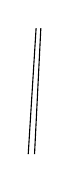
\begin{tikzpicture}\draw (0,0)--(.1,1.6);\draw (.08,0)--(.16,1.6);\end{tikzpicture}}
Je l'avais oublié dans les axiomes préliminaires il me semble, \unsure{que}\newline
\unsure{je n'} \unsure{d'avais des} \unsure{vrais} \illegible{1}

\scanpage{84}
% archive foliation: 83
Enfin, si $X=\bigoplus_{1\leq i\leq r}X_i$, la décomposition de $\Gamma^*(X)$ en \deleted{les} $\bigotimes\Gamma^*(X_i)$ donne \deleted{\unsure{une}} décomposition des $\unsure{\mathcal P|P}_n(\prod X_i;Y)$ en des $\unsure{\mathcal P|P}_{\nu_1,\ldots,\nu_r}(X_1,\ldots,X_r,Y)$.
On vérifie alors les axiomes c) à g), et le fait que \deleted{\unsure{il y a}} les produits tensoriels de $\unsure{\mathcal P|P}_1$ sont \uline{stricts} pour $\unsure{\mathcal P|P}$ (\unsure{vis} quelc. des facteurs), que les $\Gamma^{\nu_i}$ existent et satisfont la condition énoncée précédemment\ldots
\figure{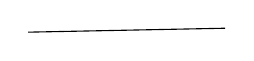
\begin{tikzpicture}\draw (0,0)--(2.5,.05);\end{tikzpicture}}
Une catégorie polynomiale $\unsure{\mathcal P|P}$ est dite \uline{stricte} si elle satisfait aux conditions préliminaires permettant de définir $\otimes$ et $\Gamma^*$ avec toutes les propriétés envisagées. D'autre part, une cat additive $\unsure{\mathcal P|P}_1$ avec $\otimes$ et $\Gamma^*$ avec les structures décrites, est dite une $\otimes$-pd-catégorie. Les deux notions sont donc en équivalence.

On dit que $\unsure{\mathcal P|P}$ est \deleted{\unsure{$k$-li}} une catégorie polynomiale (resp $\otimes$pd-cat) $k$-linéaire ($k$ anneau comm) si on a donné un hom d'anneau
\[k\longrightarrow\operatorname{End}(\mathrm{Id}_{\unsure{\mathcal P|P}_1})\quad(\unsure{\subset\mathrm{id}_\unsure{\mathcal P|P}|\in\mathrm{id}_\unsure{\mathcal P|P}}).\]

\scanpage{85}
% archive foliation: 84
tel que la décomposition de $\unsure{\mathcal P|P}_n(X_1\times\cdots\times X_r;Y)$ en des $\unsure{\mathcal P|P}_{\nu_1,\ldots,\nu_r}(X_1,\ldots,X_r;Y)$ respecte les op. de $k$, i.e. $f\in \unsure{\mathcal P|P}_{\nu_1,\ldots,\nu_r}$ implique
\[f\circ(\mathrm{id}_{\lambda_1}\times\cdots\times\mathrm{id}_{\lambda_r})=\lambda_1^{\nu_1}\cdots\lambda_r^{\nu_r}f\]
pour tt $(\lambda_1,\ldots,\lambda_r)\in k^r$.
\figure{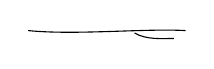
\begin{tikzpicture}\draw (0,0) .. controls (.6,-.06) and (1.5,.03) .. (2,0);\draw (1.35,-.03) .. controls (1.5,-.12) and (1.7,-.10) .. (1.85,-.10);\end{tikzpicture}}
\uline{Ex} La catégorie des $k$-modules est une $\otimes$-pd-catégorie.
De $\unsure{\Rightarrow}$ si $\unsure{\mathcal X|\mathcal T}$ un topos avec une $k$-Algèbre $K$, la cat. des $K$-Modules
\deleted{et \unsure{on p.}} [De $\unsure{\Rightarrow}$ on peut prendre des $K$-Modules gradués, \deleted{par un groupe} quelconque, \deleted{\unsure{compléter}} on \unsure{considère} des \unsure{pu. div.} $\Gamma^n(M^i)$ pour le degré $ni$.]
\margin{?}
\figure{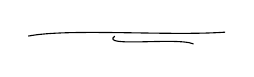
\begin{tikzpicture}\draw (0,0) .. controls (.5,.1) and (1.8,0) .. (2.5,.05);\draw (1.1,0) .. controls (.9,-.15) and (1.9,-.01) .. (2.1,-.1);\end{tikzpicture}}
Il y a diverses questions dans le cas ``abstrait''. Par exemple : quand et comment mettre sur $\Gamma^*(M)$ \inserted{($\forall M\in\operatorname{Ob}(\unsure{\mathcal P|P}_1)$)} une structure ``à p.d.'' ? i.e. des hom de degré $1$
\[\Gamma^p(\Gamma^q(M))\mathbin{-}\Gamma^{pq}(M)\]
satisfaisant aux axiomes des p.d. ?

\scanpage{86}
% archive foliation: 85
Il y a une telle structure canonique dans le cas de l'exemple.
Ou aussi : quand peut-on enrichir la composition des morphismes de $\unsure{\mathcal P|P}$
\[\deleted{\operatorname{Hom}_\unsure{\mathcal P|P}}\unsure{\mathcal P|P}(X,Y)\times \unsure{\mathcal P|P}(Y,Z)\mathbin{-}\unsure{\mathcal P|P}(X,Z)\]
($k$-linéaire en le deuxième argument) en une application linéaire
\[\unsure{\mathcal P|P}(Y,Z)\longrightarrow(\text{Appl. }k\text{-polynomiales})(\unsure{\mathcal P|P}(X,Y),\unsure{\mathcal P|P}(X,Z))\]
(ceci aussi est acquis dans l'exemple \unsure{principal} envisagé). La construction doit se ramener pour l'essentiel à définir de telles structures suppl. sur les foncteurs $\Gamma^n$, i.e. pour tt $X,Y$
\[f\longmapsto\Gamma^p(f):\operatorname{Hom}_1(X,Y)\mathbin{-}\operatorname{Hom}_1(\Gamma^pX,\Gamma^pY)\]
doit être défini comme ``application pol. de degré $p$'' entre les $k$-modules $\operatorname{Hom}_1(X,Y)$ et $\operatorname{Hom}_1(\Gamma^{\unsure{r|p}}X,\Gamma^{\unsure{r|p}}Y)$, et non seulement comme application ensembliste.

